\ExerciseSection

\begin{enumerate}
\def\labelenumi{\arabic{enumi})}
\tightlist
\item
  Let \(f(z) = z^n + a_1z^{n-1} + \cdots + a_{n-1}z + a_n\) be a polynomial of degree \(n\) with complex coefficients and put \(f(z) = \prod_{i=1}^{n}(z - z_i)\) . Let \(r_0 = \sup_i |z_i|\) .
\end{enumerate}

\begin{enumerate}
\def\labelenumi{\alph{enumi})}
\tightlist
\item
  Show that if the real number \(r > 0\) is such that
\end{enumerate}

\[
r ^ {n} \leqslant | a _ {1} | r ^ {n - 1} + | a _ {2} | r ^ {n - 2} + \dots + | a _ {n - 1} | r + | a _ {n} |,
\]

then \(r_0 \leqslant r\) , and deduce that

\[
r _ {0} \leqslant \sup \left(\mathrm{I}, \sum_ {k = 1} ^ {n} | a _ {k} |\right).
\]

\begin{enumerate}
\def\labelenumi{\alph{enumi})}
\setcounter{enumi}{1}
\item
  Let \((\lambda_i)_{1 \leqslant i \leqslant n}\) be a finite sequence of \(n\) real numbers \(>0\) such that \(\sum_{i=1}^{n} \lambda_i^{-1} = 1\) . Show that \(r_0 \leqslant \sup_k (\lambda_k |a_k|)^{1/k}\) {[}use \(a\) {]}.
\item
  Deduce from \(a\) ) that, if the coefficients \(a_i\) are all non-zero, we have
\end{enumerate}

\[
r _ {0} \leqslant \sup \left(2 | a _ {1} |, 2 \left| \frac {a _ {2}}{a _ {1}} \right|, \dots , 2 \left| \frac {a _ {n - 1}}{a _ {n - 2}} \right|, \left| \frac {a _ {n}}{a _ {n - 1}} \right|\right).
\]

\begin{enumerate}
\def\labelenumi{\alph{enumi})}
\setcounter{enumi}{3}
\tightlist
\item
  Deduce from a) that
\end{enumerate}

\[
r _ {0} \leqslant | a _ {1} - 1 | + | a _ {2} - a _ {1} | + \dots + | a _ {n - 1} - a _ {n} | + | a _ {n} |
\]

{[}consider the polynomial \((z - 1)f(z)]\) . Hence show that, if the \(a_i\) are all real and \(>0\) , we have

\[
r _ {0} \leqslant \sup \left(a _ {1}, \frac {a _ {2}}{a _ {1}}, \dots , \frac {a _ {n - 1}}{a _ {n - 2}}, \frac {a _ {n}}{a _ {n - 1}}\right).
\]

\begin{enumerate}
\def\labelenumi{\arabic{enumi})}
\setcounter{enumi}{1}
\tightlist
\item
  An algebraic number is a complex number which is algebraic over the field \(\mathbf{Q}\) of rational numbers. Show that the ordered field \(\mathbf{B}\) of all real algebraic numbers is a maximal ordered field, but that it is not complete in the topology induced by that of \(\mathbf{R}\) {[}this topology is the same as \(\mathcal{C}_0(\mathbf{B})\) ; cf.~Chapter IV, § 3, Exercise 2 b){]}.
\end{enumerate}

¶ 3) a) Let K be a maximal ordered field, endowed with the topology \(\mathfrak{G}_{0}(\mathbf{K})\) , which is compatible with its field structure (Chapter IV, § 3, Exercise 2). Let

\[
f (\mathbf {X}) = a _ {0} \mathbf {X} ^ {n} + a _ {1} \mathbf {X} ^ {n - 1} + \dots + a _ {n}
\]

be a polynomial in K{[}X{]} which has a simple root \(\alpha\) in K. Show that, for every element \(\varepsilon > 0\) in K, there exists \(\eta > 0\) in K such that every polynomial \(g(\mathbf{X}) = b_{0}\mathbf{X}^{n} + b_{1}\mathbf{X}^{n-1} + \cdots + b_{n}\) , for which \(|a_{i} - b_{i}| \leqslant \eta\) for all i, has exactly one simple root \(\beta\) such that \(|\beta - \alpha| \leqslant \varepsilon\) . (Expand f and g in powers of X - \(\alpha\) .) Give an upper bound for \(\eta\) in terms of the \(a_{i}, \alpha\) and \(\varepsilon\) .

\begin{enumerate}
\def\labelenumi{\alph{enumi})}
\setcounter{enumi}{1}
\item
  Deduce that, if K is a maximal ordered field, its completion \(\hat{K}\) with respect to \(\mathcal{G}_{0}(K)\) (which is a field with a natural order structure: Chapter IV, § 4, Exercise 2) is a maximal ordered field.
\item
  Let \(K_{0}\) be an ordered field and let \(S = K_{0}((X))\) be the field of formal power series in one indeterminate over \(K_{0}\) ; linearly order S by taking the elements \(\geqslant 0\) in S to be o and the formal power series whose term of lowest degree has coefficient \textgreater0. Show that S, endowed with the topology \(\mathcal{G}_{0}(S)\) , is complete, but that S is not a maximal ordered field (show that the polynomials \(Y^{p} - X\) of S{[}Y{]} are irreducible for each integer p \textgreater{} I).
\end{enumerate}

\(d\) ) In the example of \(c\) ), take \(\mathbf{K}_0 = \mathbb{R}\) . Let \(\mathbf{K}\) be a maximal ordered algebraic extension of \(\mathbf{S}\) ; show that \(\mathbf{K}\) is not complete in the topology \(\mathfrak{C}_0(\mathbf{K})\) . (Embed \(\mathbf{S}\) in the field \(\mathbf{E}\) of formal power series with well-ordered exponents, ordered in the same manner as \(\mathbf{S}\) , and embed \(\mathbf{K}\) in a maximal ordered extension \(\Omega\) of \(\mathbf{E}\) . Observe that \(\mathbf{E}\) is complete, and give an example of a Cauchy sequence in \(\mathbf{K}\) which converges to an element \(f \in \mathbf{E}\) which is not algebraic over \(\mathbf{S}\) ; choose \(f\) so that there is an infinite number of S-isomorphisms of \(\mathbf{E}\) into an algebraic closure of \(\Omega\) , such that the images of \(f\) under these isomorphisms are all distinct.{]}

\begin{enumerate}
\def\labelenumi{\arabic{enumi})}
\setcounter{enumi}{3}
\tightlist
\item
  Show that every continuous homomorphism (necessarily injective) \(f\) of the topological field \(\mathbf{C}\) onto a subfield of \(\mathbf{C}\) is either the identity automorphism or the automorphism \(z \to \overline{z}\) . {[}Note that we must have \(f(x) = x\) for all \(x \in \mathbf{Q}\) , and deduce that \(f(x) = x\) for all \(x \in \mathbf{R}\) .{]} Show that there exist an infinite number of discontinuous isomorphisms of \(\mathbf{C}\) onto subfields of \(\mathbf{C}\) other than \(\mathbf{C}\) itself.
\end{enumerate}

¶ 5) a) Let K be a non-commutative division subring of the division ring of quaternions H; show that the centre Z of K is a subfield of the centre R of H. (Observe that every element of K commutes with every element of the field L generated by Z ∪ R; if Z ⊕ R, the field L would be a maximal subfield of H, and K would be contained in L, contrary to hypothesis.)

\begin{enumerate}
\def\labelenumi{\alph{enumi})}
\setcounter{enumi}{1}
\tightlist
\item
  Deduce that every isomorphism \(f\) (not necessarily continuous) of \(\mathbf{H}\) onto a division subring of \(\mathbf{H}\) is an inner automorphism \(x \to axa^{-1}\) of \(\mathbf{H}\) . {[}The restriction of \(f\) to \(\mathbf{R}\) is an isomorphism of \(\mathbf{R}\) onto a subfield of \(\dot{\mathbf{R}}\) , by virtue of \(a\) ); use Exercise 3 of Chapter IV, § 3.{]}
\end{enumerate}

\ExerciseSection

\begin{enumerate}
\def\labelenumi{\arabic{enumi})}
\item
  Let \(a\) be a non-zero complex number, and \(n\) an integer \(>0\) . For each real number \(r > 0\) such that \(r^n \leqslant |a|\) , show that there exists \(z \in \mathbf{C}\) such that \(|z| = r\) and \(|a + z^n| = |a| - r^n\) . Deduce that, if \(f\) is a polynomial of degree \(>0\) , with complex coefficients, we cannot have \(|f(z_0)| \leqslant |f(z)|\) at all points \(z\) of a neighbourhood of a point \(z_0\) , provided that \(f(z_0) \neq 0\) .
\item
  Show that, if \(f\) is any polynomial with complex coefficients, not identically zero, there exists a real number \(r > 0\) such that
\end{enumerate}

\[
\left| f (z) \right| > \left| f (\mathbf {o}) \right|
\]

whenever \(|z| \geqslant r\) . Hence, with the help of Exercise 1 and Weierstrass' theorem (Chapter IV, § 6, no. 1, Theorem 1), give another proof of the fact that \(\mathbf{C}\) is algebraically closed (consider the function \(f\) on the compact set of points \(z\) such that \(|z| \leqslant r\) ).

\begin{enumerate}
\def\labelenumi{\arabic{enumi})}
\setcounter{enumi}{2}
\item
  Show, without using Theorem 1, that the mapping \(z \to z / \overline{z}\) is a strict morphism of the topological group \(\mathbf{C}^*\) onto the topological group \(\mathbf{U}\) . Deduce that the mapping \(t \to (\mathrm{i} + it) / (\mathrm{i} - it) \left[ (\mathrm{i} + it) / (\mathrm{i} - it) = -\mathrm{i} \right.\) if \(t = \infty\) is an isomorphism of the topological group \(\tilde{\mathbf{R}}\) (no. 6) onto the topological group \(\mathbf{U}\) , and hence give another proof of Theorem 1.
\item
  Let K be the smallest Pythagorean subfield of R and let \(\mathrm{K}^{\prime}=\mathrm{K}(i)\) . Let G be the multiplicative group of elements of \(K^{\prime}\) of absolute value i (a subgroup of U). Show that G is not isomorphic to the additive group of numbers of K mod i. (Observe that in the latter group there exist elements of any prime order p; on the other hand, if p is a prime such that p-1 is not a power of 2, show that G contains no pth root of unity other than 1, by noting that the degree over Q of every element of \(K^{\prime}\) is a power of 2.)
\end{enumerate}

\ExerciseSection

¶ 1) For every finite sequence \(s = (z_k)_{k \in \mathbf{I}}\) of complex numbers, put

\[
\sum_ {k \in \mathbf {I}} | z _ {k} | = \rho_ {s} \cdot \sup _ {\mathbf {J} \subset \mathbf {I}} \left| \sum_ {k \in \mathbf {J}} z _ {k} \right|
\]

(cf.~Chapter VII, § 3, no. 1, Proposition 2).

\begin{enumerate}
\def\labelenumi{\alph{enumi})}
\tightlist
\item
  * If \(z_{k} = r_{k} (\cos \varphi_{k} + i \sin \varphi_{k})\) , where \(r_{k} = |z_{k}|\) and \(\varphi_{k}\) is the principal radian measure of the amplitude of \(z_{k}\) , put
\end{enumerate}

\[
f (\varphi) = \sum_ {k \in \mathbf {I}} r _ {k} (\cos (\varphi - \varphi_ {k})) ^ {+}
\]

for every \(\varphi \in [0, 2\pi[\) . Show that the least upper bound of \(f(\varphi)\) in the interval \([0, 2\pi[\) is equal to \(\sup_{J \subset I} \left| \sum_{k \in J} z_k \right|\) . By considering the integral \(\int_0^{2\pi}f(\varphi)d\varphi\) , deduce that for all finite sequences \(s\) we have \(\rho_{s}\leqslant \pi\) and that there is no finite sequence \((z_k) = s\) such that \(\rho_{s} = \pi\)

\begin{enumerate}
\def\labelenumi{\alph{enumi})}
\setcounter{enumi}{1}
\tightlist
\item
  Show that, for every \(\varepsilon > 0\) , there exists a finite sequence \((z_k) = s\) such that \(\rho_s > \pi - \varepsilon\) (take the \(z_k\) to be the roots of a binomial equation of sufficiently high degree). *
\end{enumerate}

\begin{enumerate}
\def\labelenumi{\arabic{enumi})}
\setcounter{enumi}{1}
\tightlist
\item
  Let \((z_{n})\) be an infinite sequence of complex numbers \(z_{n} = x_{n} + iy_{n}\) such that \(x_{n} \geqslant 0\) for all \(n\) . Show that if the series whose general terms are \(z_{n}\) and \(z_{n}^{2}\) are convergent, then the series whose general term is \(z_{n}^{2}\) is absolutely convergent. Give an example in which this result is false when the condition \(x_{n} \geqslant 0\) (which can also be written \(-\pi / 2 \leqslant \operatorname{Am}(z_{n}) \leqslant \pi / 2\) ) is replaced by
\end{enumerate}

\[
- (\mathrm{I} - \varepsilon) \frac {\pi}{2} \leqslant \operatorname{Am} (z _ {n}) \leqslant (\mathrm{I} + \varepsilon) \frac {\pi}{2}
\]

no matter how small the real number \(\varepsilon > 0\) may be. (Here Am \((z)\) denotes that radian measure of the amplitude of \(z_{n}\) which belongs to the interval \([- \pi, +\pi]\) .)

\begin{enumerate}
\def\labelenumi{\arabic{enumi})}
\setcounter{enumi}{2}
\item
  Let \((z_{t})_{t\in I}\) be a family of complex numbers such that \(\prod_{t\in I}|z_t| = +\infty\) , (resp. \(\prod_{t\in I}|z_t| = 0\) ). Show that the family \((z_{t})\) is multipliable in the space \(\tilde{\mathbf{C}}\) ( \(\S 4\) , no. 3) and that its product is \(\infty\) (resp. 0).
\item
  Show that the infinite product whose general factor is \(1 + i/n\) is not convergent, but that the product of the absolute values of its factors is absolutely convergent.
\item
  Let \((z_{n})\) be an infinite sequence of non-zero complex numbers such that \(\lim_{n\to \infty}z_n = 1\) . Show that, if there exist permutations \(\sigma\) of \(\mathbf{N}\) such that the infinite product whose general factor is \(z_{\sigma (n)}\) is convergent, then the set of products
\end{enumerate}

\[
\underset {n = 0} {\overset {\infty} {\mathbf {P}}} z _ {\sigma (n)}
\]

corresponding to all these permutations can be (i) a single point; or (ii) the whole group \(\mathbf{C}^*\) ; or (iii) an open ray with origin \(\mathbf{o}\) ; or (iv) a circle with centre \(\mathbf{o}\) ; or (v) a ``logarithmic spiral'', the image of \(\mathbf{R}\) under the mapping \(t \to a^{t - t_0} (\cos t + i \sin t)\) , where \(a\) is a real number \(>0\) and \(\neq 1\) . (Argue as in Exercise 2 of Chapter VII, § 3, using the fact that the multiplicative group \(\mathbf{C}^*\) is isomorphic to the additive group \(\mathbf{R} \times \mathbf{T}\) .)

\ExerciseSection

\begin{enumerate}
\def\labelenumi{\arabic{enumi})}
\item
  Let \(f\) be a polynomial in \(n\) complex variables, with complex coefficients and not identically zero. Show that the complement in \(\mathbf{C}^n\) of the set \(S\) of points \(z = (z_i)\) such that \(f(z_1, z_2, \ldots, z_n) = 0\) (the ``algebraic variety'' with equation \(f = 0\) ) is connected. (If \(a, b\) are two distinct points of \(\mathbb{C}S\) , consider the intersections of \(S\) and the complex line through \(a\) and \(b\) .)
\item
  Let K be a non-discrete Hausdorff topological division ring (or field).
\end{enumerate}

\begin{enumerate}
\def\labelenumi{\alph{enumi})}
\tightlist
\item
  Let E be a left vector space of dimension n over K. If \((a_{i})_{1\leqslant i\leqslant n}\) is a basis of E, and if we transport to E the topology of \(K^{n}\) (the product of the topologies of the factors) by means of the bijective linear mapping
\end{enumerate}

\[
(x _ {i}) \rightarrow \sum_ {i = 1} ^ {n} x _ {i} a _ {i},
\]

then the topology so defined on E is independent of the basis \((a_{i})\) chosen, is compatible with the additive group structure of E, and is such that the mapping \((t, x) \to tx\) of \(K \times E\) into E is continuous. If F is a vector subspace of E, the topology induced on F by that of E is the same as the topology defined on F by starting from an arbitrary basis of F, as above; F is closed in E, and CF is dense in E unless F = E.

\begin{enumerate}
\def\labelenumi{\alph{enumi})}
\setcounter{enumi}{1}
\tightlist
\item
  Generalize Propositions 4, 5 and 6 of Chapter VI, § 1 to the division ring K. (To show that the mapping \(X \to X^{-1}\) is continuous in the neighbourhood of every nonsingular square matrix of order n over K, when K is not commutative, use induction on n: considering a neighbourhood of the unit matrix \(I_{n}\) of order n, note that every matrix X sufficiently near to \(I_{n}\) can be put in the form
\end{enumerate}

\[
\left( \begin{array}{c c c c} \mathrm{I} & \mathrm{O} & \ldots & \mathrm{O} \\ \lambda_ {2} & & & \\ \vdots & & I _ {n - 1} & \\ \lambda_ {n} & & & \end{array} \right) \left( \begin{array}{c c c c} \mu_ {1} & \mu_ {2} & \ldots & \mu_ {n} \\ \mathrm{o} & & & \\ \vdots & & Y & \\ \mathrm{o} & & & \end{array} \right),
\]

where \(I_{n-1}\) is the unit matrix of order n---i and Y is a nonsingular matrix of order n---i.)

\begin{enumerate}
\def\labelenumi{\alph{enumi})}
\setcounter{enumi}{2}
\item
  If K is commutative and E is an algebra of rank n over K, then the topology of E is compatible with its ring structure. Furthermore, if E has an identity element, the group G of units of E is open and dense in E, and the topology induced on G by that of E is compatible with the group structure of G. (If e is the identity element of E, and if x is a unit of E, then each of the equations xy = e, yx = e has one and one only solution y; for each of these equations consider the equivalent system of n linear equations which give the components of y with respect to a basis of E.)
\item
  If K is a non-complete field and E an algebra of rank n over K, and if the completion \(\hat{K}\) of K is a field, then the completion \(\hat{E}\) of the algebra E is that obtained by extending the ring of operators of E to \(\hat{K}\) . Hence construct examples of a topological division ring whose completion is not a division ring.
\end{enumerate}

\begin{enumerate}
\def\labelenumi{\arabic{enumi})}
\setcounter{enumi}{2}
\item
  Using Proposition 10 of Chapter I, § 3, no. 6, prove that the real projective space \(\mathbf{P}_{n}(\mathbf{R})\) is homeomorphic to the subspace of \(\mathbf{P}_{n}(\mathbf{C})\) consisting of these points which have at least one system of real homogeneous coordinates. \([\mathbf{R}_{n+1}^{*}\) being considered as embedded in \(\mathbf{C}_{n+1}^{*}\) , let A be a closed set in \(\mathbf{R}_{n+1}^{*}\) , saturated with respect to \(\Delta_{n}(\mathbf{R})\) ; let B be the set of all points \(\zeta x\) , where \(x \in A\) and \(\zeta \in U\) ; show that \(\overline{\mathbf{B}}\) is saturated with respect to \(\Delta_{n}(\mathbf{C})\) , and that A is the trace of \(\overline{\mathbf{B}}\) on \(\mathbf{R}_{n+1}^{*}\) .{]}
\item
  In \(\mathbf{P}_{n}(\mathbf{C})\) let \(H_{n}\) be the ``quadric'' defined by the equation
\end{enumerate}

\[
x _ {0} ^ {2} + x _ {1} ^ {2} + \dots + x _ {n} ^ {2} = 0.
\]

Show that every point of \(H_{n}\) has an open neighbourhood homeomorphic to \(C^{n-1}\) , that \(H_{n}\) is connected, and that the intersection of \(H_{n}\) with the complement of any complex projective hyperplane is connected (to prove this last assertion, reduce to the case \(n = 2\) ).

Show that \(H_{2}\) is homeomorphic to \(S_{2}\) , and \(H_{3}\) to \(S_{2} \times S_{2}\) (use the parametric representation of the quadric by means of its rectilinear generators).

\begin{enumerate}
\def\labelenumi{\arabic{enumi})}
\setcounter{enumi}{4}
\tightlist
\item
  The sphere \(\mathbf{S}_5\) being considered as a subspace of \(\mathbf{C}^3\) , consider the mapping of \(\mathbf{S}_5\) into \(\mathbf{R}^7\) which sends each point \(x = (x_1, x_2, x_3)\) of \(\mathbf{S}_5\) ( \(x_1, x_2, x_3\) complex) to the point \(y = (y_i)_{1 \leqslant i \leqslant 7}\) of \(\mathbf{R}^7\) , where
\end{enumerate}

\[
\begin{array}{c} y _ {1} = | x _ {1} | ^ {2} - | x _ {2} | ^ {2}, \quad y _ {2} = \mathcal {R} (x _ {1} \overline {{x}} _ {2}), \quad y _ {3} = \mathcal {I} (x _ {1} \overline {{x}} _ {2}), \quad y _ {4} = \mathcal {R} (x _ {1} \overline {{x}} _ {3}), \\ y _ {5} = \mathcal {I} (x _ {1} \overline {{x}} _ {3}), \quad y _ {6} = \mathcal {R} (x _ {2} \overline {{x}} _ {3}), \quad y _ {7} = \mathcal {I} (x _ {2} \overline {{x}} _ {3}). \end{array}
\]

This function has the same value at two points \(\pmb{x}, \pmb{x}'\) of \(\mathbf{S}_5\) such that \(\pmb{x}' = \zeta \pmb{x}\) , where \(|\zeta| = 1\) . Show that, by passing to the quotient, it induces a homeomorphism of \(\mathbf{P}_2(\mathbf{C})\) onto a subspace of \(\mathbf{R}^7\) .

¶ 6) Let K be a non-discrete Hausdorff topological division ring (or field).

\begin{enumerate}
\def\labelenumi{\alph{enumi})}
\tightlist
\item
  Endow the left projective space \(\mathbf{P}_n(\mathbf{K})\) with the quotient of the topology of \(\mathbf{K}_{n+1}^*\) by the equivalence relation \(\Delta_n(\mathbf{K})\) . Extend Propositions 1, 4 and 5 of Chapter VI, § 3, to \(\mathbf{P}_n(\mathbf{K})\) endowed with this topology. Show that \(\mathbf{P}_n(\mathbf{K})\) is connected if \(\mathbf{K}\) is connected, and otherwise is totally disconnected.
\end{enumerate}

* b) If K is locally compact (but not discrete), show that \(\mathbf{P}_{n}(\mathbf{K})\) is compact. (Let U be a compact neighbourhood of o in K; let \(a \in K\) be such that

\[
\lim _ {m \rightarrow \infty} a ^ {m} = 0;
\]

let S be the subset of \(K_{n+1}^{*}\) consisting of points \(\boldsymbol{x} = (x_{i})\) , all of whose coordinates \(x_{i}\) belong to U, and such that \(x_{k} \in a\) . \(\overline{U}\) for some index k; show that \(\mathbf{P}_{n}(\mathbf{K})\) is the canonical image of S). *

\begin{enumerate}
\def\labelenumi{\alph{enumi})}
\setcounter{enumi}{2}
\item
  Likewise, extend Definition 2 and Propositions 6 and 8 of Chapter VI, § 3 to the set \(\mathbf{P}_{n,p}(\mathbf{K})\) of projective linear varieties of \(p\) dimensions in \(\mathbf{P}_n(\mathbf{K})\) ; * also Proposition 7, assuming that \(\mathbf{K}\) is locally compact {[}for Proposition 7 consider, for each sequence \(\sigma\) of indices, the subset \(\mathrm{S}_{\sigma}\) of \(\mathrm{A}_{\sigma}\) consisting of matrices all of whose rows belong to the set S defined in \(b\) ); show that \(\mathbf{P}_{n,p}(\mathbf{K})\) is the canonical image of the union of the sets \(\mathrm{S}_{\sigma}]\) . * Generalize Proposition 9 of Chapter VI, § 3, when \(\mathbf{K}\) is a field.
\item
  If K is not commutative, let \(\mathbf{P}_{n,p}^{\prime}(\mathbf{K})\) denote the space of p-dimensional projective linear varieties in the right projective space of n dimensions over K {[}the topology of \(\mathbf{P}_{n,p}^{\prime}(\mathbf{K})\) being defined in the same way as that of \(\mathbf{P}_{n,p}(\mathbf{K})\) {]}. Show that \(\mathbf{P}_{n,p}(\mathbf{K})\) and \(\mathbf{P}_{n,n-p-1}^{\prime}(\mathbf{K})\) are homeomorphic {[}to every \((p+1)\) -dimensional vector subspace V of the left vector space \(E=K_{s}^{n+1}\) make correspond the orthogonal complement of V, which is a vector subspace of the dual \(E^{*}\) of E{]}.
\end{enumerate}

\begin{enumerate}
\def\labelenumi{\arabic{enumi})}
\setcounter{enumi}{6}
\item
  Extend Exercise 6 of Chapter VI, § 3 to spaces of projective linear varieties over C and H.
\item
  Extend Exercises 7, 8 and 9 of Chapter VI, § 3 to the spaces \(\mathbf{W}_{n,p}\) (no. 4).
\end{enumerate}

In the vector space \(H^{n}\) over the division ring of quaternions, we again denote by \(W_{n,p}\) the set of all sequences \((x_{k})_{1\leqslant k\leqslant p}\) of p vectors \(x_{k}=(x_{kj})_{1\leqslant j\leqslant n}\) such that

\[
\sum_ {j = 1} ^ {n} x _ {i j} \overline {{{x}}} _ {i j} = \mathrm{I} \quad (\mathrm{I} \leqslant i \leqslant p)
\]

and

\[
\sum_ {j = 1} ^ {n} x _ {i j} \bar {x} _ {i j} = 0 \quad (i \neq k)
\]

( \(\bar{x}\) denoting the conjugate of the quaternion \(x\) ). Extend Exercises 7, 8 and 9 of Chapter VI, § 3, to these spaces \(\mathbf{W}_{n,p}\) .

\section*{HISTORICAL NOTE}
\phantomsection
\addcontentsline{toc}{section}{Historical Note}

(Numbers in brackets refer to the bibliography at the end of this note.)

We shall not repeat here the complete history of the development of the theories of complex numbers and quaternions, since these theories belong essentially to algebra; but we shall say something about the geometrical representation of complex numbers, which in many respects was a decisive step forward in the history of mathematics.

Without any doubt the first to have a clear conception of the one-to-one correspondence between complex numbers and points in the plane was C. F. Gauss (*), who moreover applied this idea to the theory of complex numbers and foresaw the uses to which it would be put by the analysts of the 19th century. During the 17th and 18th centuries, mathematicians had gradually come to the conviction that imaginary numbers, which allowed them to solve all quadratic equations, could also be used to solve algebraic equations of any degree. Many attempts to prove this theorem were published during the course of the 18th century; but, not mentioning those which were based only on a vicious circle, there was not one which was not open to serious objection. Gauss, after a detailed examination of these attempts and a closely reasoned criticism of their deficiencies, proposed in his inaugural dissertation (written in 1797, published in 1799) to give at last a rigorous proof. Taking up an idea thrown off in passing by d'Alembert {[}in his proof published in 1746 (**){]},

Gauss remarked that the points \((a, b)\) of the plane which are such that \(a + ib\) is a root of the polynomial \(\mathrm{P}(x + iy) = \mathrm{X}(x, y) + i\mathrm{Y}(x, y)\) are the intersections of the curves X = o and Y = o; by means of a qualitative study of these curves, he then shows that a continuous arc of one of them joins points of two distinct regions bounded by the other, and concludes from this that the curves intersect ({[}1{]}, vol.~3, p.~3; see also {[}1 a{]}). In its clarity and originality this proof was a considerable advance on previous attempts, and was certainly one of the first examples of purely topological reasoning applied to a problem of algebra (*).

In his dissertation, Gauss does not explicitly define the correspondence between points of the plane and complex numbers; as to the latter, and the questions of ``existence'' to which they had given rise for two hundred years, he reserves his position and deliberately presents all his arguments in a form which involves only real quantities. But the march of ideas in his proof would be wholly unintelligible if it did not presuppose a fully conscious identification of points of the plane with complex numbers; and his research at the same period in number theory and elliptic functions, which also involve complex numbers, reinforces this supposition. The way in which the geometrical conception of imaginaries became familiar to him, and the results it could lead to in his hands, are clearly shown by the notes (published only recently) in which he applies complex numbers to the solution of problems of elementary geometry ({[}1{]}, vol.~4, p.~396 and vol.~8, p.~307). Even more explicit is the letter to Bessel in 1811 ({[}1{]}, vol.~8, p.~90-91) in which he sketches the essentials of the theory of integration of functions of a complex variable: ``Just as the whole domain of real quantities can be represented by means of an infinite line, so the complete domain of all quantities, both real and imaginary, can be realized by means of an infinite plane, in which each point, determined by its abscissa a and its ordinate b, represents at the same time the quantity \(a + ib\) . The continuous passage from one value of x to another consequently takes place along a curve, and can therefore be achieved in an infinity of ways\ldots''.

But it was not until 1831 that Gauss (à propos the introduction of ``Gaussian integers'' \(a + ib\) , where \(a\) and \(b\) are integers) publicly expounded his ideas on this point so precisely ({[}1{]}, vol.~2, Theoria Residuorum Biquadraticorum, Commentatis Secunda, art. 38, p.~109, and Anzeige, p.~174 et seq.). In the intervening years, the idea of representing complex numbers geometrically had been independently rediscovered by two modest amateurs, both of them more or less self-taught, who made no other contribution to mathematics, and who were both without much contact with the scientific circles of their time. For this reason their work was in danger of passing completely unnoticed; this is precisely what happened to the first in point of date, a pamphlet written by a Dane, C. Wessel. Published in 1798, it was clearly conceived and written, but was not rescued from oblivion until a century later. The same mishap might have overtaken the second, by the Swiss J. Argand, who owed it only to chance that he saw his work, published in 1806, exhumed seven years later (*). This work provoked an active discussion in the Annales de Gergonne, and was the subject, in France and England, of several publications by obscure authors between 1820 and 1830. But the authority of a great name was needed to put an end to these controversies and to rally mathematicians to the new point of view, and it was not until the middle of the century that the geometrical representation of complex numbers at last became universally adopted, following the publications of Gauss (mentioned above) in Germany, the work of Hamilton and Cayley on hypercomplex systems in England, and finally the support of Cauchy (** ) in France, only a few years before the genius of Riemann was to extend still further the role of geometry in the theory of analytic functions, and at the same stroke create the science of topology.

\par\noindent\textbf{* \(\ast\)}\par

The measurement of angles by means of the arcs they cut off on a circle is as old as the notion of angle itself, and was already known to the Babylonians: their unit of angular measure was the degree, which we still use. The Babylonians used only measures of angles lying between o and 360°; this was adequate for their purposes, which were primarily to fix the positions of celestial objects at determinate points of their apparent orbits and to construct tables of these orbits for scientific or astrological purposes.

Among the Greek geometers of the classical era, the notion of angle (Euclid's Elements, I, Definitions 8 and 9) was even more restricted, because it applied only to angles smaller than two right angles; and since on the other hand their theory of proportion and measurement was based on the comparison of arbitrarily large multiples of the magnitudes being measured, angles could not be measurable quantities for them, although of course they had the concepts of equal angles, of one angle being greater or less than another, and of the sum of two angles, provided that the sum did not exceed two right angles. Just as with the addition of fractions, the measurement of angles must have been in their eyes an empirical procedure, devoid of scientific value. This attitude is well illustrated by the admirable essay of Archimedes on spirals ({[}3{]}, vol.~2, pp.~1-121) in which, since he cannot define them by the proportionality of radius vector to angle, he gives a kinematic definition (Definition 1, p.~44; cf.~the statement of Proposition 12, p.~46) from which he succeeds in extracting, as the rest of the work shows, everything that the general notion of angular measure would have given him had he been in possession of it. As to the Greek astronomers, they seem to have been content to follow their Babylonian predecessors on this point as on many others.

Here too, as in the evolution of the concept of real number (cf.~the Historical Note on Chapter IV), the relaxation of the spirit of rigour during the decadence of Greek science brought a return to the ``naive'' point of view which, in some respects, comes nearer to our own than does the rigid Euclidean conception. Thus an ill-advised interpolator inserted the following famous proposition in Euclid (Euclid's Elements, VI, 33): ``Angles are proportional to the arcs which they cut out on a circle'' (*), and an anonymous scholar who comments on the ``proof'' of this proposition does not hesitate to introduce, of course without justification, arcs equal to arbitrarily large multiples of a circumference, and the angles corresponding to these arcs (**). But even Vietà, in the 16th century, although he appeared to come close to our modern conception of angle when he discovered that the equation \(\sin nx = \sin \alpha\) has several roots, obtained only those roots corresponding to angles smaller than two right angles ({[}4{]}, p.~305). Only in the 17th century was this point of view definitively superseded; and, after the discovery by Newton of the power-series expansions for \(\sin x\) and \(\cos x\) had furnished expressions of these functions which were valid for all values of the variable, Euler finally formulated the precise conception of the notion of angular measure, in connection with logarithms of ``imaginary'' numbers ({[}5{]}, (1), vol.~17, p.~220).

Of course, the classical definition of angular measure in terms of the length of a circular arc is not only intuitive but essentially correct; however it requires, to make it rigorous, the notion of the length of a curve, i.e., integral calculus. From the point of view of the structures which come into play, this is a very long-winded procedure, and it is possible, as we have seen in the text, to arrive at the same end by no other means than those of the theory of topological groups; in this manner the real exponential and the complex exponential appear as arising from the same source, the theorem which characterizes the ``one-parameter groups'' (Chapter V, § 3, Theorem 1).

\subsection*{BIBLIOGRAPHY}

{[}1{]} C. F. Gauss, Werke, vol.~2 (2nd edition, Göttingen, 1876); vol.~3 (2nd edition, ibid., 1876); vol.~4 (ibid., 1873) and vol.~8 (ibid., 1900).

{[}1 a{]} Die vier Gauss'schen Beweise für die Zerlegung ganzer algebraischer Functionen in reelle Factoren ersten oder zweiten Grades {[}Ostwald's Klassiker, no. 14, Leipzig (Teubner), 1904{]}.

{[}2{]} Euclidis Elementa, 5 vols., edited by J. L. Heiberg, Leipzig (Teubner) 1883-1888.

{[}3{]} Archimedis Opera Omnia, 3 vols., vol.~2, pp.~1-121, edited by J. L. Heiberg, 2nd edition, Leipzig (Teubner) 1913-15.

{[}3 a{]} Les Œuvres complètes d'Archimède, translated by P. Ver Eecke, Paris-Brussels (Desclée de Brouwer), 1921.

{[}4{]} FRANCISCI VIETAE, Opera Mathematica, p.~305, Leyden (Bonaventure et Abraham Elzevir), 1646.

{[}5{]} L. EULER, Opera omnia (1), vol.~17, p.~220, Leipzig (Teubner), 1915.

\chapter{Use of real numbers in general topology}

\section{GENERATION OF A UNIFORMITY BY A FAMILY OF PSEUDOMETRICS; UNIFORMIZABLE SPACES}

\subsection{PSEUDOMETRICS}

DEFINITION 1. If X is a set, a pseudometric on X is any mapping f of X × X into the interval {[}0, +∞{]} of the extended real line R which satisfies the following conditions:

\((\mathrm{EC}_{\mathbf{I}})\) For all \(x \in \mathbf{X}, f(x, x) = 0\) .

\((\mathrm{EC}_{\mathrm{II}})\) For all \(x \in \mathbf{X}\) and all \(y \in \mathbf{X}, f(x, y) = f(y, x)\) (symmetry). \((\mathrm{EC}_{\mathrm{III}})\) For all \(x, y, z\) in \(\mathbf{X}\) ,

\[
f (x, y) \leqslant f (x, z) + f (z, y)
\]

(triangle inequality).

Examples. 1) On real number space \(\mathbf{R}^n\) , Euclidean distance (Chapter VI, § 2, no. 1) is a pseudometric.

\begin{enumerate}
\def\labelenumi{\arabic{enumi})}
\setcounter{enumi}{1}
\item
  If X is any set, the function f defined on \(X \times X\) by the conditions \(f(x, x) = 0\) for all \(x \in X\) , \(f(x, y) = +\infty\) if \(x \neq y\) is a pseudometric on X.
\item
  If \(\mathbf{X}\) is any set and if \(g\) is any finite real-valued function defined on \(\mathbf{X}\) , then the function \(f\) defined on \(\mathbf{X} \times \mathbf{X}\) by \(f(x, y) = |g(x) - g(y)|\) is a pseudometric on \(\mathbf{X}\) .
\end{enumerate}

* 4) Let X be the set of all continuous mappings of the interval {[}0, 1{]} of R into R. If for each pair of elements x, y of X we put

\[
f (x, y) = \int_ {0} ^ {1} | x (t) - y (t) | d t,
\]

then \(f\) is a pseudometric on \(\mathbf{X}\) . *

Remarks. 1) Example 2 above shows that a pseudometric can take the value +∞ for certain pairs of elements of X.

\begin{enumerate}
\def\labelenumi{\arabic{enumi})}
\setcounter{enumi}{1}
\tightlist
\item
  If \(f\) is a pseudometric on \(\mathbf{X}\) , we can in general have \(f(x, y) = 0\) without \(x = y\) , as Example 3 above shows (cf.~§ 2).
\end{enumerate}

From the triangle inequality it follows that if \(f(x, z)\) and \(f(y, z)\) are finite then so is \(f(x, y)\) ; moreover, in this case we have

\[
f (x, z) \leqslant f (y, z) + f (x, y) \quad \text { and } \quad f (y, z) \leqslant f (x, z) + f (x, y),
\]

so that

\[
\left| f (x, z) - f (y, z) \right| \leqslant f (x, y).\tag{1}
\]

If \(f\) is a pseudometric on \(\mathbf{X}\) , then so is \(\lambda f\) for any finite real number \(\lambda > 0\) . If \((f_t)_{t \in I}\) is any family of pseudometrics on \(\mathbf{X}\) , the sum \(\sum_{i \in I} f_i(x, y)\) is defined for all \((x, y) \in \mathbf{X} \times \mathbf{X}\) ; if \(f(x, y)\) denotes the value of this sum, then \(f\) is a pseudometric on \(\mathbf{X}\) . Again, the upper envelope \(g\) of the family \((f_t)\) (Chapter IV, § 5, no. 5) is a pseudometric on \(\mathbf{X}\) , for the relations \(f_i(x, y) \leqslant f_i(x, z) + f_i(z, y)\) imply

\[
\sup _ {t \in I} f _ {t} (x, y) \leqslant \sup _ {t \in I} \left(f _ {t} (x, z) + f _ {t} (z, y)\right) \leqslant \sup _ {t \in I} f _ {t} (x, z) + \sup _ {t \in I} f _ {t} (z, y)
\]

{[}Chapter IV, § 5, no. 7, formula (17){]}.

\subsection{DEFINITION OF A UNIFORMITY BY MEANS OF A FAMILY OF PSEUDOMETRICS}

We have seen in Chapter VI, § 2, no. 3 that if, for each real number \(a > 0\) , we denote by \(\mathbf{U}_a\) the set of all pairs \((x, y)\) of points of \(\mathbf{R}^n\) whose Euclidean distance apart is \(\leqslant a\) , then the \(\mathbf{U}_a\) form a fundamental system of entourages of the uniformity of \(\mathbf{R}^n\) as \(a\) runs through the set of real numbers \(> 0\) .

More generally, let \(f\) be a pseudometric on a set \(\mathbf{X}\) ; for each \(a > 0\) , let \(\mathbf{U}_a\) denote \(\overline{f}^{1}([o, a])\) , and let us show that, as \(a\) runs through the set of all real numbers \(> 0\) , the \(\mathbf{U}_a\) form a fundamental system of entourages of a uniformity on \(\mathbf{X}\) . Axiom \((\mathbf{U}_{\mathbf{I}}^{\prime})\) is satisfied by reason of \((\mathrm{EC}_{\mathbf{I}})\) ; if \(a \leqslant b\) , we have \(\mathbf{U}_a \subset \mathbf{U}_b\) and therefore the \(\mathbf{U}_a\) satisfy \((\mathbf{B}_{\mathbf{I}})\) ; by \((\mathrm{EC}_{\mathbf{II}})\) , we have \(\overline{\mathbf{U}}_a = \mathbf{U}_a\) and therefore \((\mathbf{U}_{\mathbf{II}}^{\prime})\) is satisfied; finally, by \((\mathrm{EC}_{\mathbf{III}})\) we have \(\overline{\mathbf{U}}_a \subset \mathbf{U}_{2a}\) , so that \((\mathbf{U}_{\mathbf{III}}^{\prime})\) is satisfied. {[}Cf. Chapter II, § 1, no. 1, Definition 2{]}. Consequently we may make the following definition:

DEFINITION 2. Given a pseudometric \(f\) on a set \(\mathbf{X}\) , the uniformity defined by \(f\) is the uniformity on \(\mathbf{X}\) which has as a fundamental system of entourages the family of sets \(\overline{f}^{1}([0, a])\) , where a runs through the set of all real numbers \(> 0\) .

Two pseudometrics on X are said to be equivalent if they define the same uniformity.

Remarks. 1) If \((a_{n})\) is any sequence of numbers \(>0\) and tending to \(0\) , the \(\mathrm{U}_{a_n}\) form a fundamental system of entourages of the uniformity defined by \(f\) .

\begin{enumerate}
\def\labelenumi{\arabic{enumi})}
\setcounter{enumi}{1}
\tightlist
\item
  The definition of a uniformity by a pseudometric \(f\) consists in taking as a fundamental system of entourages the inverse image under \(f\) of the neighbourhood filter of \(o\) in the subspace \([o, +\infty]\) of \(\overline{\mathbf{R}}\) . Note that this procedure is quite analogous to that which allowed us to define the uniformities on a topological group (Chapter III, § 3, no. 1).
\end{enumerate}

Let \(f\) and \(g\) be two pseudometrics on \(\mathbf{X}\) . From Definition 2 it follows that the uniformity defined by \(f\) is coarser than the uniformity defined by \(g\) if and only if, for each \(a > 0\) there exists \(b > 0\) such that the relation \(g(x, y) \leqslant b\) implies \(f(x, y) \leqslant a\) . A necessary and sufficient condition for \(f\) and \(g\) to be equivalent pseudometrics is that for each \(a > 0\) there exists \(b > 0\) such that \(g(x, y) \leqslant b\) implies \(f(x, y) \leqslant a\) , and \(f(x, y) \leqslant b\) implies \(g(x, y) \leqslant a\) .

In particular, if there exists a constant \(k\) such that \(f \leqslant kg\) , the uniformity defined by \(f\) is coarser than the uniformity defined by \(g\) .

Let \(\varphi\) be a mapping of the interval \([o, +\infty]\) into itself, satisfying the following conditions: 1) \(\varphi(o) = o\) , and \(\varphi\) is continuous at \(o\) ; 2) \(\varphi\) is increasing in \([o, +\infty]\) and is strictly increasing in a neighbourhood of \(o\) ; 3) for all \(u \geqslant o\) and \(v \geqslant o\) , we have \(\varphi(u + v) \leqslant \varphi(u) + \varphi(v)\) . Then if \(f\) is any pseudometric on a set X, the composition \(g = \varphi \circ f\) is a pseudometric equivalent to \(f\) .

The reader may easily verify that we may, for example, take \(\varphi\) to be any one of the following functions:

\[
\sqrt {u}, \quad \log (\mathrm{I} + u), \quad \frac {u}{\mathrm{I} + u}, \quad \inf (u, \mathrm{I}).
\]

The last two examples show that there always exist bounded pseudometrics equivalent to any given pseudometric (finite or not).

DEFINITION 3. If \((f_{t})_{t\in I}\) is a family of pseudometrics on a set \(X\) , then the least upper bound of the set of uniformities defined on \(X\) by the pseudometrics \(f_{t}\) is called the uniformity defined by the family \((f_{t})\) .

Two families of pseudometrics on X are said to be equivalent if they define the same uniformity on X.

From the definition of the least upper bound of a set of uniformities (Chapter II, § 2, no. 5), the filter of entourages of the uniformity U defined on X by a family of pseudometrics \((f_{t})_{t\in\mathbf{I}}\) is the filter generated (Chapter I, §6, no. 2) by the family of sets \(\overline{f}_{t}^{1}([o,a])\) , where t runs through I and a runs through the set of real numbers \textgreater0. In other words, we obtain a fundamental system of entourages of U by proceeding as follows: we take at random a finite number of indices \(\iota_{1},\iota_{2},\ldots,\iota_{n}\) and, corresponding to each \(\iota_{k}\) , a number \(a_{k}>0\) ; then we consider the set V of pairs \((x,y)\in\mathbf{X}\times\mathbf{X}\) such that \(f_{\iota_{k}}(x,y)\leqslant a_{k}\) for \(i\leqslant k\leqslant n\) ; these sets V (for all possible choices of n, the \(\iota_{k}\) and the \(a_{k}\) ) form a fundamental system of entourages for U. Moreover, we may restrict ourselves to the case in which all the \(a_{k}\) are equal to the same number a\textgreater0, since the entourage consisting of all pairs \((x,y)\) such that

\[
\sup _ {1 \leqslant k \leqslant n} \left(f _ {\iota_ {k}} (x, y)\right) \leqslant \inf _ {1 \leqslant k \leqslant n} a _ {k}
\]

is evidently contained in V.

For each finite subset H of I, let \(g_{H}\) denote the upper envelope of the family \((f_{t})_{t\in\mathbb{H}}\) . As H runs through the set of all finite subsets of I and a runs through the set of real numbers \textgreater0, the sets \(g_{\mathrm{H}}^{-1}([o,a])\) form a fundamental system of entourages of the uniformity U. Now the \(g_{H}\) are pseudometrics on X (no. 1), and the upper envelope of a finite number of functions of the family \((g_{\mathrm{H}})\) belongs to this family, by definition; we express this property by saying that the family of pseudometrics \((g_{\mathrm{H}})\) is saturated. The family of pseudometrics \((g_{\mathrm{H}})\) is therefore equivalent to the family \((f_{t})\) , and is said to be the family of pseudometrics obtained by saturating \((f_{t})\) . From what has just been said it follows that we may always restrict ourselves to considering uniformities defined by saturated families of pseudometrics.

In the particular case where \(\mathbf{I}\) is a finite set, this argument shows that the uniformity defined by the family of pseudometrics \((f_{t})_{t\in \mathbf{I}}\) is also defined by the single pseudometric \(g = \sup_{t\in \mathbf{I}}f_t\) .

Let \(\mathcal{U},\mathcal{U}'\) be two uniformities on \(\mathbf{X}\) , defined respectively by two saturated families \((f_{t})_{t\in \mathbf{I}},(g_{x})_{x\in \mathbf{K}}\) . Then \(\mathcal{U}\) is coarser than \(\mathcal{U}'\) if and only if, for each index \(t\in I\) and each real number \(a > 0\) , there is an index \(x\in K\) and a number \(b > 0\) such that the relation \(g_{x}(x,y)\leqslant b\) implies \(f_{t}(x,y)\leqslant a\) .

Example of a uniformity defined by a family of pseudometrics. Let \((f_{t})_{t\in I}\) be an arbitrary family of (finite) real-valued functions defined on a set \(X\) . Let \(\mathcal{U}\) be the coarsest uniformity on \(X\) with respect to which the \(f_{t}\) are uniformly continuous (Chapter II, § 2, no. 3). Then it follows from the definition of the entourages of \(\mathcal{U}\) (loc. cit.) that \(\mathcal{U}\) is the uniformity defined on \(X\) by the pseudometrics

\[
g _ {i} (x, y) = | f _ {i} (x) - f _ {i} (y) |.
\]

\subsection{PROPERTIES OF UNIFORMITIES DEFINED BY FAMILIES OF PSEUDOMETRICS}

Let \(\mathcal{U}\) be a uniformity defined on a set \(X\) by a family of finite pseudometrics \((f_{i})\) . If we endow \(X \times X\) with the uniformity which is the product of \(\mathcal{U}\) by itself, then each of the real-valued functions \(f_{i}\) is uniformly continuous on \(X \times X\) ; for by (1) we have

\[
\left| f _ {t} (x, y) - f _ {t} \left(x ^ {\prime}, y ^ {\prime}\right) \right| \leqslant f _ {t} (x, x ^ {\prime}) + f _ {t} (y, y ^ {\prime}),
\]

and therefore the relations \(f_{i}(x, x') \leqslant \varepsilon / 2\) , \(f_{i}(y, y') \leqslant \varepsilon / 2\) imply

\[
\left| f _ {t} (x, y) - f _ {t} \left(x ^ {\prime}, y ^ {\prime}\right) \right| \leqslant \varepsilon .
\]

For \(\mathcal{U}\) to be Hausdorff it is necessary and sufficient, from the definition of the entourages of \(\mathcal{U}\) , that for each pair of distinct points \(x, y\) of \(\mathbf{X}\) there is an index \(\iota\) such that \(f_{\iota}(x, y) \neq 0\) .

In particular, if \(\mathcal{U}\) is defined by a single pseudometric \(f\) , then \(\mathcal{U}\) is Hausdorff if and only if the relation \(f(x,y)=0\) implies \(x=y\) (cf.~§ 2). If \(\mathcal{U}\) is not Hausdorff, the intersection of all the entourages of \(\mathcal{U}\) is the subset of \(\mathbf{X} \times \mathbf{X}\) consisting of pairs \((x,y)\) such that \(f_{i}(x,y)=0\) for all \(\iota\) ; this subset is the graph of an equivalence relation \(\mathbf{R}\) on \(\mathbf{X}\) , and the Hausdorff uniformity associated with \(\mathcal{U}\) is defined on \(\mathbf{X}/\mathbf{R}\) (cf.~Chapter II, § 3, no. 8). It is then easily verified that the functions \(f_{i}\) are compatible (in \(x\) and in \(y\) ) with the relation \(\mathbf{R}\) (Set Theory, \(\mathbf{R}\) , § 5, no. 7) and that the functions \(\overline{f_{i}}\) , obtained from \(f_{i}\) by passing to the quotient (with respect to \(x\) and \(y\) ), are pseudometrics on \(\mathbf{X}/\mathbf{R}\) which define the Hausdorff uniformity associated with \(\mathcal{U}\) (cf.~§ 2, no. 1).

If A is a non-empty subset of X, the restriction to \(A \times A\) of a pseudometric on X is clearly a pseudometric on A. The uniformity induced by U on A is clearly that defined by the family of restrictions to \(A \times A\) of the pseudometrics \(f_{t}\) .

Let us now look at the completion of the uniform space \(\mathbf{X}\) when \(\mathcal{U}\) is Hausdorff.

PROPOSITION 1. Let X be a Hausdorff uniform space whose uniformity U is defined by a family of finite pseudometrics ( \(f_{t}\) ), and let \(\hat{X}\) be the completion of X. Then the functions \(f_{t}\) can be extended by continuity to \(\hat{\mathbf{X}} \times \hat{\mathbf{X}}\) ; the extended functions \(\overline{f_t}\) are finite pseudometrics on \(\hat{\mathbf{X}} \times \hat{\mathbf{X}}\) , and the family \((f_{t})\) defines the uniformity of \(\hat{\mathbf{X}}\) .

First, the \(f_{t}\) can be extended by continuity to \(\hat{\mathbf{X}}\times\hat{\mathbf{X}}\) , because they are uniformly continuous on \(\mathbf{X}\times\mathbf{X}\) ; and the extended functions \(\overline{f_{t}}\) are uniformly continuous on \(\hat{\mathbf{X}}\times\hat{\mathbf{X}}\) (Chapter II, § 3, no. 6, Theorem 2); moreover, they are pseudometrics on \(\hat{\mathbf{X}}\) by virtue of the principle of extension of inequalities (Chapter IV, § 5, no. 2, Theorem 1). Let \(\mathcal{U}_{1}\) denote the uniformity on \(\hat{\mathbf{X}}\) obtained by completion, and let \(\mathcal{U}_{2}\) denote the uniformity defined by the family of pseudometrics ( \(\overline{f_{t}}\) ). Then \(\mathcal{U}_{2}\) is coarser than \(\mathcal{U}_{1}\) ; for each \(\overline{f_{t}}\) is uniformly continuous on \(\hat{\mathbf{X}}\times\hat{\mathbf{X}}\) with respect to \(\mathcal{U}_{1}\) , and hence for each \(a>0\) there exists an entourage V of \(\mathcal{U}_{1}\) such that, whenever \((x,y)\in\mathrm{V}\) , we have \(|\overline{f_{t}}(x,y)-\overline{f_{t}}(x,x)|\leqslant a\) , that is {[}since \(\overline{f_{t}}(x,x)=0\) {]}, \(\mathrm{V}\subset\overline{f_{t}}([0,a])\) ; hence every entourage of \(\mathcal{U}_{2}\) is an entourage of \(\mathcal{U}_{1}\) . On the other hand, \(\mathcal{U}_{1}\) and \(\mathcal{U}_{2}\) induce the same uniformity \(\mathcal{U}\) on X. As \(\hat{\mathbf{X}}\) is complete with respect to \(\mathcal{U}_{1}\) , it follows that \(\mathcal{U}_{1}\) and \(\mathcal{U}_{2}\) are identical (Chapter II, § 3, no. 7, Proposition 14).

\subsection{CONSTRUCTION OF A FAMILY OF PSEUDOMETRICS DEFINING A UNIFORMITY}

The significance of defining a uniformity by means of a family of pseudometrics lies in the fact that all uniformities can be so obtained. Namely:

THEOREM 1. Given a uniformity \(\mathcal{U}\) on a set \(X\) , there is a family of pseudometrics on \(X\) such that the uniformity defined by this family is identical with \(\mathcal{U}\) .

For each entourage V of the uniformity U, define inductively a sequence of symmetric entourages \((\mathbf{U}_{n})\) such that \(U_{1} \subset V\) and \(\dot{U}_{n+1}^{2} \subset U_{n}\) for all \(n \geqslant 1\) . The sequence \((\mathbf{U}_{n})\) is a fundamental system of entourages of a uniformity \(U_{v}\) coarser than U; moreover, it is clear that U is the least upper bound of all the uniformities \(U_{v}\) as V runs through the filter of entourages of U. Theorem 1 is therefore a consequence of the following proposition:

PROPOSITION 2. If a uniformity U on X has a countable fundamental system of entourages, then there is a pseudometric f on X such that U is identical with the uniformity defined by f.

Let \((\mathbf{V}_n)\) be a countable fundamental system of entourages of \(\mathcal{U}\) . Define inductively a sequence \((\mathbf{U}_n)\) of symmetric entourages of \(\mathcal{U}\) such that \(\mathbf{U}_1 \subset \mathbf{V}_1\) and

\[
\mathbf {\dot {U}} _ {n + 1} ^ {3} \subset \mathbf {U} _ {n} \cap \mathbf {V} _ {n} \quad \text {   for   } \quad n \geqslant 1.
\]

Clearly \((\mathbf{U}_n)\) is another fundamental system of entourages of \(\mathcal{U}\) , and we have in particular \(\dot{\mathbf{U}}_{n+1}^3 \subset \mathbf{U}_n\) for \(n \geqslant 1\) . We define a real-valued function \(g\) on \(\mathbf{X} \times \mathbf{X}\) as follows: \(g(x, y) = 0\) if \((x, y) \in \mathbf{U}_n\) for all \(n\) ; \(g(x, y) = 2^{-k}\) if \((x, y) \in \mathbf{U}_n\) for \(1 \leqslant n \leqslant k\) , but \((x, y) \notin \mathbf{U}_{k+1}\) ; \(g(x, y) = 1\) if \((x, y) \notin \mathbf{U}_1\) . The function \(g\) is symmetric and positive, and we have \(g(x, x) = 0\) for all \(x \in \mathbf{X}\) . Put

\[
f (x, y) = \inf \sum_ {i = 0} ^ {p - 1} g \left(z _ {i}, z _ {i + 1}\right),
\]

the greatest lower bound being taken over the set of all finite sequences \((z_{i})_{0\leqslant i\leqslant p}\) ( \(p\) arbitrary) such that \(z_0 = x\) and \(z_{p} = y\) . We shall show that \(f\) is a pseudometric which satisfies the inequalities

\[
\frac {1}{2} g (x, y) \leqslant f (x, y) \leqslant g (x, y).\tag{2}
\]

It follows immediately from the definition that \(f\) is symmetric and positive and satisfies the triangle inequality. Also it is clear that \(f(x, y) \leqslant g(x, y)\) , hence \(f(x, x) = 0\) for all \(x \in \mathbf{X}\) , and therefore \(f\) is a pseudometric. To prove the left-hand half of the inequalities (2), let us show by induction on \(p\) that, for every finite sequence \((z_i)_{0 \leqslant i \leqslant p}\) of \(p + 1\) points of \(\mathbf{X}\) such that \(z_0 = x\) and \(z_p = y\) , we have

\[
\sum_ {i = 0} ^ {p - 1} g (z _ {i}, \quad z _ {i + 1}) \geqslant \frac {\mathrm{I}}{2} g (x, y).\tag{3}
\]

This is clear if \(p = \mathbf{i}\) . Put \(a = \sum_{i=0}^{p-1} g(z_i, z_{i+1})\) ; the inequality (3) is true if \(a \geqslant \mathbf{i}/2\) , because \(g(x, y) \leqslant \mathbf{i}\) . Suppose then that \(a < \mathbf{i}/2\) , and let \(h\) be the largest of the indices \(q\) such that

\[
\sum_ {i <   q} g (z _ {i}, z _ {i + 1}) \leqslant \frac {a}{2};
\]

we have then \(\sum_{i < h} g(z_i, z_{i+1}) \leqslant a/2\) and \(\sum_{i < h+1} g(z_i, z_{i+1}) > a/2\) , whence

\[
\sum_ {i > h} g (z _ {i}, z _ {i + 1}) \leqslant \frac {a}{2}.
\]

By the inductive hypothesis we have \(g(x, z_h) \leqslant a\) and \(g(z_{h+1}, y) \leqslant a\) ; on the other hand it is clear that \(g(z_h, z_{h+1}) \leqslant a\) . Let \(k\) be the smallest integer \(> 0\) such that \(2^{-k} \leqslant a\) ; then \(k \geqslant 2\) , and \((x, z_h) \in \mathbf{U}_k\) , \((z_h, z_{h+1}) \in \mathbf{U}_k\) , \((z_{h+1}, y) \in \mathbf{U}_k\) by the definition of \(g\) ; hence \((x, y) \in \mathbf{U}_k \subset \mathbf{U}_{k-1}\) , which implies that \(g(x, y) \leqslant 2^{1-k} \leqslant 2a\) .

Hence the inequalities (2) are proved; they show that, for each \(a > 0\) , the set \(\overline{f}^{1}([o, a])\) contains \(\mathbf{U}_{k}\) for each index \(k\) such that \(2^{-k} < a\) , and conversely that each \(\mathbf{U}_{k}\) contains the set \(\overline{f}^{1}([o, 2^{-k-1}])\) ; hence the sets \(\overline{f}^{1}([o, a])\) form a fundamental system of entourages of the structure \(\mathfrak{U}\) .

Remark. A uniformity \(\mathfrak{U}\) on \(\mathbf{X}\) is defined by the family \(\Phi\) of all pseudometrics on \(\mathbf{X}\) which are uniformly continuous on \(\mathbf{X} \times \mathbf{X}\) . For clearly the uniformity defined by the family \(\Phi\) is coarser than \(\mathfrak{U}\) ; conversely, Theorem 1 shows that there is a subfamily of \(\Phi\) which defines the uniformity \(\mathfrak{U}\) and therefore the uniformity defined by \(\Phi\) is finer than \(\mathfrak{U}\) .

\subsection{UNIFORMIZABLE SPACES}

In Chapter II, § 4, no. 1, we posed the problem of characterizing uniformizable topological spaces. The solution is given by the following theorem:

THEOREM 2. A topological space X is uniformizable if and only if it satisfies the following axiom:

\((\mathrm{O}_{\mathrm{IV}})\) Given any point \(x_0 \in X\) and any neighbourhood \(V\) of \(x_0\) , there exists a continuous real-valued function on \(X\) which takes its values in \([0,1]\) , is equal to 0 at \(x_0\) , and is equal to 1 on CV.

The condition is necessary. For if there is a uniformity on X compatible with the topology of X, then by Theorem 1 this uniformity can be defined by a family \((f_{t})\) of pseudometrics on X, and we may assume with no loss of generality that this family is saturated (no. 2). From the definition of the entourages of the uniformity defined by such a family of pseudometrics, there is a pseudometric \(f_{\alpha}\) of the family \((f_{t})\) , and a number \(a > 0\) , such that \(f_{\alpha}(x_0, x) \geqslant a\) for all \(x \in \mathbb{C}\mathrm{V}\) . It follows that the function \(g(x) = \inf \left(1, \frac{1}{a} f_{\alpha}(x_0, x)\right)\) satisfies all the conditions laid down in \((\mathrm{O}_{\mathrm{IV}})\) .

The condition is sufficient. For let \(\Phi\) be the set of all continuous mappings of X into {[}o, i{]}. Axiom (O \(_{IV}\) ) shows that the coarsest uniformity with respect to which all the functions belonging to \(\Phi\) are uniformly continuous is compatible with the topology of X (Chapter II, § 2, no. 3).

DEFINITION 4. A topological space is said to be completely regular if it is uniformizable and Hausdorff.

Equivalently, in view of Theorem 2, a space is completely regular if it satisfies axioms (H) {[}cf.~Chapter I, § 8, no. 1, Proposition 1{]} and \((\mathbf{O}_{\mathbf{IV}})\) .

Remark. Axiom \((\mathrm{O}_{\mathrm{IV}})\) implies \((\mathrm{O}_{\mathrm{III}})\) (cf.~Chapter I, § 8, no. 4), for if V is a neighbourhood of \(x_0\) and if \(f\) is a continuous real-valued function on X with values in {[}o, r{]}, such that \(f(x_0) = o\) , \(f(x) = 1\) for all \(x \in \complement V\) , then the set \(\overline{f}([0, 1/2])\) is a closed neighbourhood of \(x_0\) contained in V. In particular, every completely regular space is regular (which justifies the terminology). But there are examples of regular spaces which are not completely regular (*), so that \((\mathrm{O}_{\mathrm{III}})\) does not imply \((\mathrm{O}_{\mathrm{IV}})\) .

Every compact space is completely regular (Chapter II, § 4, no. 1, Theorem 1) and therefore so is every subspace of a compact space. We can now complete this proposition by proving its converse:

PROPOSITION 3. A topological space X is completely regular if and only if it is homeomorphic to a subspace of a compact space.

Consider the coarsest uniformity on X with respect to which all continuous mappings of X into {[}o, 1{]} are uniformly continuous; we have already used this uniformity in the proof of Theorem 2, where we saw that it is compatible with the topology of X if X is uniformizable. Furthermore, this uniformity is a structure of a precompact space, by the compactness of the interval {[}o, 1{]} and Proposition 3 of Chapter II, § 4, no. 2. If X is Hausdorff, the completion of X with respect to this is therefore compact, and the proposition is proved.

We can therefore say that a completely regular space can be embedded in a compact space. It is often convenient to present this result in the following way:

In general, a cube is a topological space \(K^{I}\) , the product of a family of topological spaces each identical with a compact interval K of R, indexed by an arbitrary set I. If I is finite and has n elements, we recover the notion of an n-dimensional closed cube, which was defined in Chapter VI, § 1, no. 1. A cube is a compact space (Chapter I, § 9, no. 5, Theorem 3).

PROPOSITION 4. If a topological space X is completely regular, it is homeomorphic to a subspace of a cube.

Let \((f_{i})_{i\in \mathbf{I}}\) denote the family of all continuous mappings of \(\mathbf{X}\) into \(\mathbf{K} = [\mathrm{o},\mathrm{i}]\) , and let \(g\) denote the mapping \(x\to (f_i(x))\) of \(\mathbf{X}\) into

\(K^{I}\) . If x, y are any two distinct points of X, it follows from axioms (H) and \((\mathrm{O}_{\mathrm{IV}})\) that there is an index t such that \(f_{t}(x) \neq f_{t}(y)\) , and therefore g is a one-to-one mapping of X into \(K^{I}\) . Moreover, it is immediate that g is an isomorphism of the coarsest uniformity on X for which all the \(f_{t}\) are uniformly continuous, onto the uniformity induced on \(g(\mathbf{X})\) by the product uniformity of \(K^{I}\) ; a fortiori, g is a homeomorphism of X onto \(g(\mathbf{X})\) .

\subsection{SEMI-CONTINUOUS FUNCTIONS ON A UNIFORMIZABLE SPACE}

In Chapter IV, § 6, no. 2, Corollary to Theorem 4, we showed that the upper envelope of a family of continuous real-valued functions on a topological space is a lower semi-continuous function. If the space is uniformizable, there is a converse to this proposition:

PROPOSITION 5. In order that every lower semi-continuous real-valued function \(f\) (finite or not) on a topological space \(\mathbf{X}\) should be the upper envelope of the continuous real-valued functions on \(\mathbf{X}\) (finite or not) which are \(\leqslant f\) , it is necessary and sufficient that \(\mathbf{X}\) be uniformizable.

The condition is necessary. Let \(x_0\) be any point of \(\mathbf{X}\) and let \(\mathbf{V}\) be any open neighbourhood of \(x_0\) ; then the characteristic function \(\varphi_{\mathbf{V}}\) of the set \(\mathbf{V}\) is lower semi-continuous (Chapter IV, § 6, no. 2, Corollary to Proposition 1); by hypothesis, there is therefore a continuous real-valued function \(g\) on \(\mathbf{X}\) such that \(g \leqslant \varphi_{\mathbf{V}}\) and \(g(x_0) = a > 0\) . The continuous function \(\inf\left(\mathbf{i}, \frac{\mathbf{i}}{a} g^+\right)\) takes its values in {[}o, i{]}, is equal to o in CV, and equal to i at \(x_0\) . Hence (Theorem 2) \(\mathbf{X}\) is uniformizable.

The condition is sufficient. Consider first the case in which \(f\) takes its values in \([-1, +1]\) . We have to show that, for each \(x_0 \in X\) and each number \(a < f(x_0)\) , there is a continuous real-valued function \(g\) on \(X\) such that \(g \leqslant f\) and \(g(x_0) \geqslant a\) . If \(a \leqslant -1\) , we may take \(g\) to be the constant \(-1\) . If \(-1 < a < f(x_0)\) , there is a neighbourhood \(V\) of \(x_0\) such that \(f(x) \geqslant a\) for all \(x \in V\) . Since \(X\) is uniformizable, there is a continuous real-valued function \(h\) on \(X\) , with values in \([0, 1]\) , such that \(h(x_0) = 0\) and \(h(x) = 1\) for all \(x \in C_V\) . We may then take \(g(x) = a - (a + 1)h(x)\) , and we have a continuous function satisfying the stated conditions. Note that this function takes its values in \([-1, +1]\) .

The general case follows by transfer of structure; for there is a strictly increasing homeomorphism of \([-1, +1]\) onto \(\overline{R}\) (Chapter IV, § 4, no. 2, Proposition 2), and the definition of a semi-continuous function involves only the order structure and the topology of \(\overline{R}\) .

Remark. In the above proof we see that the function g does not take the value +1. By transfer of structure it follows that every lower semi-continuous real-valued function f on the uniformizable space X is the upper envelope of the continuous real-valued functions \(g \leqslant f\) on X which do not take the value +∞.

\section{METRIC SPACES AND METRIZABLE SPACES}

\subsection{METRICS AND METRIC SPACES}

DEFINITION 1. A metric on a set X is a finite pseudometric d on X such that the relation \(d(x, y) = 0\) implies x = y. A metric space is a set X endowed with the structure defined by a given metric on X.

A metric space X is always considered as carrying the uniformity and the topology defined by the given metric on X.

Examples. 1) The Euclidean distance \(d(\pmb{x}, \pmb{y})\) (Chapter VI, § 2, no. 1) is a metric on real \(n\) -dimensional number space \(\mathbf{R}^n\) ; so are the functions

\[
\sup _ {1 \leqslant i \leqslant n} | x _ {i} - y _ {i} | \quad \text { and } \quad \sum_ {i = 1} ^ {n} | x _ {i} - y _ {i} |.
\]

All these metrics are equivalent (§ 1, no. 2).

\begin{enumerate}
\def\labelenumi{\arabic{enumi})}
\setcounter{enumi}{1}
\tightlist
\item
  On any set X the pseudometric \(d\) , defined by the relations \(d(x, x) = 0\) and \(d(x, y) = 1\) if \(x \neq y\) , is a metric. The uniformity it defines on X is the discrete uniformity.
\end{enumerate}

We have a definition equivalent to Definition 1 if we say that a metric is a finite pseudometric such that the uniformity defined by this pseudometric is Hausdorff; a finite pseudometric which is equivalent to a metric is therefore a metric.

Uniform spaces defined by a single pseudometric (which we may assume to be finite) can be reduced to metric spaces when the pseudometric is not a metric. Let \(f\) be such a pseudometric on a set \(\mathbf{X}\) , and let \(\mathcal{U}\) be the uniformity defined by \(f\) ; \(\mathcal{U}\) is not Hausdorff, and the intersection of the entourages of \(\mathcal{U}\) is the subset of \(\mathbf{X} \times \mathbf{X}\) defined by the equivalence relation \(f(x,y) = 0\) . Let \(\mathbf{R}\) denote this relation. If \(x \equiv x' \pmod{\mathbf{R}}\) , then by the triangle inequality we have

\[
f (x, y) \leqslant f (x, x ^ {\prime}) + f (x ^ {\prime}, y) = f (x ^ {\prime}, y)
\]

and similarly \(f(x', y) \leqslant f(x, y)\) , so that \(f(x, y) = f(x', y)\) ; in other words, \(f\) is a function compatible (in \(x\) and \(y\) ) with the equivalence relation \(\mathbf{R}\) (Set Theory, \(\mathbf{R}\) , § 5, no. 7). Let \(\overline{f}\) be the function induced by \(f\) on the quotient set; \(\overline{f}\) is defined on \((\mathbf{X}/\mathbf{R}) \times (\mathbf{X}/\mathbf{R})\) , and if \(x\) and \(y\) are any two points of \(\mathbf{X}\) and if \(\dot{x}\) and \(\dot{y}\) denote the equivalence classes (mod \(\mathbf{R}\) ) of \(x\) and \(y\) respectively, then we have \(\overline{f}(\dot{x}, \dot{y}) = f(x, y)\) . It follows immediately that \(\overline{f}\) is a metric on \(\mathbf{X}/\mathbf{R}\) ; it is called the metric associated with the pseudometric \(f\) ; furthermore, the uniformity it defines on \(\mathbf{X}/\mathbf{R}\) is precisely the Hausdorff uniformity associated with \(\mathcal{U}\) by the definition of this uniformity (Chapter II, § 3, no. 8, Remark). Thus, by passing to a suitable quotient space, the uniform structure defined by a single pseudometric can be reduced to the structure of a metric space.

Proposition 1 of § 1, no. 3 determines the structure of the completion of a metric space:

PROPOSITION 1. Let X be a metric space and let d be its metric. If \(\hat{X}\) is the completion of X (with respect to the uniformity defined by \(d\) ), the function \(d\) can be extended by continuity to \(\hat{X} \times \hat{X}\) ; the extended function \(\overline{d}\) is a metric on \(\hat{X}\) , and the uniformity of \(\hat{X}\) coincides with that defined by the metric \(\overline{d}\) .

Proposition 1 of § 1, no. 3 shows that \(\overline{d}\) is a finite pseudometric on \(\hat{\mathbf{X}}\) , and that the uniformity defined by \(\overline{d}\) on \(\hat{\mathbf{X}}\) is the uniformity obtained by completion; since this latter uniformity is Hausdorff, \(\overline{d}\) is a metric. Whenever we consider the completion of a metric space \(\mathbf{X}\) as a metric space, it is always to be understood that the metric on \(\hat{\mathbf{X}}\) is that obtained by extending the metric on \(\mathbf{X}\) by continuity.

\subsection{STRUCTURE OF A METRIC SPACE}

Let X and \(X'\) be two metric spaces, d the metric on X, \(d'\) the metric on \(X'\) . In accordance with the general definitions (Set Theory, R, § 8, no. 5) a one-to-one mapping f of X onto \(X'\) is an isomorphism of the metric space structure of X onto that of \(X'\) if

\[
d (x, y) = d ^ {\prime} (f (x), f (y))\tag{1}
\]

for all \(x \in \mathbf{X}\) and all \(y \in \mathbf{X}\) .

Note that if \(f\) is a mapping of \(\mathbf{X}\) onto \(\mathbf{X}'\) which satisfies the identity (1), then \(f\) must be bijective and therefore an isomorphism of \(\mathbf{X}\) onto \(\mathbf{X}'\) ; such an isomorphism is also called an isometry (or an isometric mapping) of \(\mathbf{X}\) onto \(\mathbf{X}'\) .

\pandocbounded{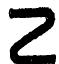
\includegraphics[keepaspectratio]{images/part001_40fd7be3.jpg}}

An isometry of X onto \(X'\) is of course an isomorphism of the uniformity (resp. topology) of X onto the uniformity (resp. topology) of \(X'\) ; the converses of these statements are false, as is shown by the existence of distinct equivalent metrics ( \(\S\) 1, no. 2).

Let X be a metric space, d the metric on X. For each a \textgreater{} 0 let \(V_{a}\) denote the subset of \(X \times X\) consisting of all pairs \((x, y)\) such that \(d(x, y) < a\) , and let \(W_{a}\) denote the subset of \(X \times X\) consisting of all pairs \((x, y)\) such that \(d(x, y) \leqslant a\) . As a runs through the set of all real numbers \textgreater{} 0 (or merely a sequence of numbers \textgreater{} 0 which tends to 0), the sets \(V_{a}\) (resp. \(W_{a}\) ) form a fundamental system of open (resp. closed) entourages of the uniformity of X, because of the continuity of d (§ 1, no. 3). We have \(\overline{V}_{a} \subset W_{a}\) , but these two sets are not necessarily the same.

By analogy with the case of the Euclidean distance on \(R^{n}\) , the set \(\mathrm{V}_{a}(x)\) {[}resp. \(\mathrm{W}_{a}(x)\) {]} is called the open (resp. closed) ball with centre x and radius a; it is an open (resp. closed) set in X. Again, the set of all \(y \in X\) such that \(d(x, y) = a\) is called the sphere with centre x and radius a; it is a closed set. From what has been said, the open (resp. closed) balls with centre x and radius a form a fundamental system of neighbourhoods of x as a runs through the set of all real numbers \textgreater0, or a sequence of numbers \textgreater0 which tends to o.

\pandocbounded{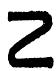
\includegraphics[keepaspectratio]{images/part001_d95d2d33.jpg}}

The reader should beware of assuming that balls and spheres in an arbitrary metric space enjoy the same properties as the Euclidean balls and spheres studied in Chapter VI, § 2. Thus the closure of an open ball need not be the closed ball of the same centre and radius; the frontier of a closed ball need not be the sphere of the same centre and radius; an open (or closed) ball need not be connected; and a sphere can be empty (cf.~Exercise 4).

Let A and B be any two non-empty subsets of a metric space X. The number

\[
d (\mathbf {A}, \mathbf {B}) = \inf _ {x \in \mathbf {A}, y \in \mathbf {B}} d (x, y)
\]

is called the distance between the sets A and B. In particular we denote by \(d(x, \mathbf{A})\) the distance between the set \(\{x\}\) and the set A; this is called the distance from the point x to the set A. Thus

\[
d (x, \mathrm{A}) = \inf _ {y \in \mathrm{A}} d (x, y)
\]

whence

\[
d (\mathbf {A}, \mathbf {B}) = \inf _ {x \in \mathbf {A}} d (x, \mathbf {B})
\]

(Chapter IV, § 5, no. 4, Proposition 9).

Remark. If \(d(x, \mathrm{A}) = a\) , it can happen that there is no point of A whose distance from \(x\) is equal to \(a\) . However, this situation can never arise if A is compact, for then Weierstrass's theorem (Chapter IV, §6, no. 1, Theorem 1) shows that there exists \(y \in \mathrm{A}\) such that \(d(x, \mathrm{A}) = d(x, y)\) .

PROPOSITION 2. The statements \(d(x, \mathbf{A}) = 0\) and \(x \in \overline{\mathbf{A}}\) are equivalent.

For \(d(x, \mathbf{A}) = 0\) expresses the fact that the ball \(\mathbf{V}_a(x)\) meets \(\mathbf{A}\) whatever the value of \(a > 0\) ; and this is equivalent to \(x \in \overline{\mathbf{A}}\) .

PROPOSITION 3. The function \(d(x, \mathbf{A})\) is uniformly continuous on \(\mathbf{X}\) .

Let \(x\) and \(y\) be any two points of \(\mathbf{X}\) ; then given any \(\varepsilon > 0\) there exists \(z \in \mathbf{A}\) such that \(d(y, z) \leqslant d(y, \mathbf{A}) + \varepsilon\) , and therefore

\[
d (x, z) \leqslant d (x, y) + d (y, z) \leqslant d (x, y) + d (y, A) + \varepsilon
\]

by the triangle inequality.

A fortiori \(d(x, \mathbf{A}) \leqslant d(x, y) + d(y, \mathbf{A}) + \varepsilon\) , and since \(\varepsilon\) is arbitrary it follows that \(d(x, \mathbf{A}) \leqslant d(x, y) + d(y, \mathbf{A})\) . Similarly we have

\[
d (y, \mathbf {A}) \leqslant d (x, y) + d (x, \mathbf {A}),
\]

so that

\[
\left| d (x, \mathbf {A}) - d (y, \mathbf {A}) \right| \leqslant d (x, y),\tag{2}
\]

whence the result follows.

Remark. We can have \(d(\mathbf{A}, \mathbf{B}) = 0\) for two subsets \(\mathbf{A}, \mathbf{B}\) of \(\mathbf{X}\) such that \(\overline{\mathbf{A}} \cap \overline{\mathbf{B}} = \emptyset\) , provided that neither subset consists of a single point. For example, on the real line \(\mathbf{R}\) , the set of integers \(> 0\) and the set of points of the sequence \((n + 1/2n)_{n \geqslant 1}\) are two disjoint closed sets whose distance apart is zero.

However, if A is compact and B is closed, the relation \(d(A, B) = 0\) implies \(A \cap B \neq \varnothing\) , for by virtue of the relation

\[
d (\mathbf {A}, \mathbf {B}) = \inf _ {x \in \mathbf {A}} d (x, \mathbf {B})
\]

it follows from Proposition 3 and Weierstrass's theorem that there exists \(x_0 \in \mathbf{A}\) such that \(d(x_0, \mathbf{B}) = d(\mathbf{A}, \mathbf{B}) = 0\) and hence (Proposition 2) \(x_0 \in \mathbf{B}\) .

The diameter of a non-empty subset A of X is the number (finite or equal to +∞)

\[
\delta (\mathbf {A}) = \sup _ {x \in \mathbf {A}, y \in \mathbf {A}} d (x, y).
\]

The notion of a ``W \(_{a}\) -small set'' (Chapter II, § 3, no. 1) is identical with that of a set of diameter \(\leqslant a\) . A non-empty set A consists of a single point if and only if \(\delta(\mathbf{A}) = 0\) .

A subset A of X is bounded (with respect to the metric d) if its diameter is finite; equivalently, if for each point \(x_{0} \in X\) , A is contained in a ball with centre \(x_{0}\) . Every subset of a bounded set is bounded, and the union of a finite family of bounded sets is a bounded set.

Note that a subset of X can be bounded with respect to a metric d but unbounded with respect to a metric equivalent to d (cf.~§ 1, no. 2).

\subsection{OSCILLATION OF A FUNCTION}

Related to the notion of diameter is that of the oscillation of a function \(f\) , defined on an arbitrary set \(\mathbf{X}\) and taking its values in a metric space \(\mathbf{X}'\) ; if \(\mathbf{A}\) is any non-empty subset of \(\mathbf{X}\) , the diameter \(\delta(f(\mathbf{A}))\) is called the oscillation of \(f\) in \(\mathbf{A}\) .

If moreover \(\mathbf{X}\) is a subset of a topological space \(\mathbf{Y}\) , and if \(x \in \overline{\mathbf{X}}\) , the number

\[
\omega (x; f) = \inf \delta (f (\mathbf {V} \cap \mathbf {X}))
\]

(as V runs through the neighbourhood filter of \(x\) in Y) is called the oscillation of \(f\) at \(x \in \overline{\mathbf{X}}\) .

PROPOSITION 4. The oscillation \(\omega(x; f)\) of an arbitrary function \(f\) , defined on a subset X of a topological space Y and taking its values in a metric space \(\mathbf{X}'\) , is upper semi-continuous on \(\overline{\mathbf{X}}\) .

Let \(a\) be any point of \(\overline{\mathbf{X}}\) ; then for each \(k > \omega(a; f)\) there exists an open neighbourhood \(\mathbf{V}\) of \(a\) such that \(\delta(f(\mathbf{V} \cap \mathbf{X})) \leqslant k\) ; for each \(x \in \mathbf{V} \cap \overline{\mathbf{X}}\) , \(\mathbf{V}\) is a neighbourhood of \(x\) and therefore

\[
\omega (x; f) \leqslant \delta (f (\mathbf {V} \cap \mathbf {X})) \leqslant k,
\]

which shows that \(\omega\) is upper semi-continuous at the point a.

In order that \(\omega(x; f) = 0\) at a point \(x \in \overline{\mathbf{X}}\) it is necessary and sufficient that for each \(\varepsilon > 0\) there should exist a neighbourhood \(\mathbf{V}\) of \(x\) such that \(f(\mathbf{V} \cap \mathbf{X})\) is contained in a ball of radius \(\varepsilon\) ; if \(x \in \mathbf{X}\) , this condition expresses the fact that \(f\) is continuous at the point \(x\) (with respect to \(\mathbf{X}\) ); if \(x \in \overline{\mathbf{X}} \cap \complement \mathbf{X}\) , the image under \(f\) of the trace on \(\mathbf{X}\) of the neighbourhood filter of \(x\) in \(\mathbf{Y}\) is a Cauchy filter base on \(\mathbf{X}'\) ; in particular:

PROPOSITION 5. Let \(f\) be a function defined on a subset \(\mathbf{X}\) of a topological space \(\mathbf{Y}\) , taking its values in a complete metric space \(\mathbf{X}'\) . Then \(f\) has a limit relative to \(\mathbf{X}\) at a point \(x \in \overline{\mathbf{X}}\) if and only if the oscillation of \(f\) at \(x\) is zero.

\subsection{METRIZABLE UNIFORM SPACES}

DEFINITION 2. A metric on a set X is said to be compatible with a uniformity U on X if the uniformity defined by the metric coincides with U.

A uniformity on a set X is said to be metrizable if there is a metric on X compatible with this uniformity. A uniform space is said to be metrizable if its uniformity is metrizable.

Distinct metrics can be compatible with the same uniformity; they are then equivalent (§ 1, no. 2, Definition 2).

THEOREM 1. A uniformity is metrizable if and only if it is Hausdorff and the filter of entourages of the uniformity has a countable base.

The condition is necessary, for (with the notation of no. 2) the entourages \(V_{1/n}\) ( \(n \geqslant 1\) ) form a base of the filter of entourages of the uniformity of a metric space.

The condition is sufficient, for, if it is satisfied, the uniformity under consideration is defined by a single pseudometric, by Proposition 2 of § 1, no. 4; since the uniformity is Hausdorff, this pseudometric is a metric.

COROLLARY 1. A Hausdorff uniformity defined by a countable family of pseudometrics is metrizable.

For if \((f_n)\) is a sequence of pseudometrics defining such a structure, the filter of entourages is generated by the countable family of sets \(\overline{f}_n^1([0, 1/m])\) , where \(m\) and \(n\) each run through the set of integers \(>0\) .

COROLLARY 2. Every countable product of metrizable uniform spaces is metrizable.

For such a space is Hausdorff and its uniformity has a countable fundamental system of entourages (Chapter II, § 2, no. 6).

\subsection{METRIZABLE TOPOLOGICAL SPACES}

DEFINITION 3. A metric on a set X is said to be compatible with a topology C on X if the topology defined by this metric coincides with C. A topological space is said to be metrizable if there exists a metric on X compatible with the topology of X.

\pandocbounded{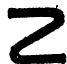
\includegraphics[keepaspectratio]{images/part001_d7e316f7.jpg}}

Two metrics on a set X which are both compatible with the same topology \(\mathfrak{C}\) can be inequivalent.

The subspace \(R_{+}^{*}\) of R provides an example of this. Both the uniformity induced by the additive uniformity of R and the uniformity induced by the multiplicative uniformity of \(R^{*}\) are metrizable and are compatible with the topology of \(R_{+}^{*}\) ; but they are not comparable.

We remark also that there can exist non-metrizable uniformities compatible with the topology of a metrizable topological space (Exercise 7).

We shall content ourselves here with necessary conditions for the metrizability of a topological space (for a necessary and sufficient condition, cf.~§ 4, Exercise 22). In the first place, a space cannot be metrizable unless it is completely regular (indeed we shall see, in § 4, no. 1, Proposition 2, that a metrizable space is necessarily ``normal'', which is a stronger condition). On the other hand, Theorem 1 shows that:

PROPOSITION 6. Every point of a metrizable space has a countable fundamental system of neighbourhoods.

More generally :

PROPOSITION 7. In a metrizable space, every closed set is the intersection of a countable family of open sets, and every open set is the union of a countable family of closed sets.

Let \(d\) be a metric compatible with the topology of a metrizable space \(\mathbf{X}\) . If \(\mathbf{A}\) is a closed subset of \(\mathbf{X}\) , it is the intersection of the open sets \(\mathrm{V}_{1/n}(\mathbf{A})\) {[}the set of all \(x\in\mathbf{X}\) such that \(d(x,\mathbf{A})<\mathbf{1}/n\) ; cf.~Proposition 2{]}. The second part of the proposition follows by taking complements.

Remarks. 1) These necessary conditions are not sufficient (cf.~Exercise 13). 2) There are spaces in which every point has a countable fundamental system of neighbourhoods but in which there exist closed sets which are not countable intersections of open sets (Exercise 15); such spaces are not metrizable.

Corollary 2 of Theorem 1, no. 4, shows that a countable product of metrizable topological spaces is metrizable. Also the sum X (Chapter I, § 2, no. 4) of an arbitrary family \((\mathbf{X}_t)_{t \in \mathbf{I}}\) of metrizable spaces is metrizable. For if \(d_t\) is a metric compatible with the topology of \(\mathbf{X}_t\) for each \(t \in \mathbf{I}\) , we may assume that \(d_t\) is bounded and that the diameter of \(\mathbf{X}_t\) is \(\leqslant t\) ; we can then define a distance \(d\) compatible with the topology of \(\mathbf{X}\) by putting \(d(x, y) = d_t(x, y)\) if \(x\) and \(y\) both belong to the same \(\mathbf{X}_t\) , and \(d(x, y) = t\) otherwise.

\subsection{USE OF COUNTABLE SEQUENCES}

Proposition 6 is the origin of the part played by countable sequences of points in the theory of metrizable spaces; for many problems, they can be used to advantage in place of filters. This is because the neighbourhood filters of points of a metrizable space (and therefore also convergent filters) are determined by convergent sequences of points of the space: for since the neighbourhood filter of a point has a countable base, it is the intersection of the elementary filters finer than itself (Chapter I, § 6, no. 8, Proposition 11), i.e., of the elementary filters associated with sequences which converge to the point in question.

On the other hand, the notion of a convergent sequence is not adapted to the study of topological spaces in which there are points whose neighbourhood filter has no countable base. In particular, Hausdorff non-discrete topological spaces can be constructed in which, at every point x, the intersection of any countable family of neighbourhoods of x is again a neighbourhood of \(x (*)\) ; in such a space the only convergent sequences are those in which all the terms are equal from a certain index onwards.

As examples of the use of countable sequences we give the following propositions:

PROPOSITION 8. In a metrizable space X, a point x lies in the closure of a non-empty subset A of X if and only if there is a sequence of points of A which converges to x.

We know already, from Chapter I, § 7, no. 3, that the condition is sufficient. To see that it is necessary, consider a countable fundamental system \((\mathbf{V}_n)\) of neighbourhoods of \(x\) such that \(\mathbf{V}_{n+1} \subset \mathbf{V}_n\) for each \(n\) . If \(x\) lies in the closure of A then each \(\mathbf{V}_n\) meets A, and if \(x_n\) lies in \(\mathbf{V}_n \cap \mathbf{A}\) , the sequence \((x_n)\) converges to \(x\) (**).

From Proposition 8 we deduce:

PROPOSITION 9. A metric space X is complete if and only if every Cauchy sequence in X is convergent.

Let \(\hat{\mathbf{X}}\) be the completion of \(\mathbf{X}\) . If there is a point \(x \in \hat{\mathbf{X}}\) which does not belong to \(\mathbf{X}\) , then there is a sequence \((x_n)\) of points of \(\mathbf{X}\) which converges to \(x\) , and this is a non-convergent Cauchy sequence in \(\mathbf{X}\) .

PROPOSITION 10. Let X be a metrizable space and let f be a mapping of X into a topological space \(X'\) . Then f is continuous at a point \(x \in X\) if and only if, whenever \((x_n)\) is a sequence of points of X which converges to x, the sequence \((f(x_n))\) converges to \(f(x)\) in \(X'\) .

The condition is necessary, from Chapter I, § 7, no. 4, Proposition 9, Corollary 1. To show that it is sufficient, consider the filter \(\mathfrak{B}'\) of neighbourhoods of \(f(a)\) in \(\mathbf{X}'\) ; the hypothesis implies that \(\overline{f}(\mathfrak{B}')\) is coarser than every elementary filter associated with a sequence which converges to \(a\) , that is to say every elementary filter which converges to \(a\) ; but the intersection of these filters is the neighbourhood filter of \(a\) (Chapter I, § 6, no. 8, Proposition 11). Hence the result.

Note that Propositions 8 and 10 are valid in any space X in which every point has a countable fundamental system of neighbourhoods.

\subsection{SEMI-CONTINUOUS FUNCTIONS ON A METRIZABLE SPACE}

PROPOSITION 11. Let X be a metrizable space and let f be a lower semicontinuous function on X which takes its values in a closed interval \([a, b]\) of \(\overline{R}\) . Then f is the upper envelope of an increasing sequence of continuous functions on X which take their values in \([a, b]\) .

By transfer of structure we may assume that \(a = 0\) and \(b = 1\) .

\begin{enumerate}
\def\labelenumi{(\roman{enumi})}
\tightlist
\item
  Suppose first that \(f = \varphi_{\mathbf{A}}\) , where \(\mathbf{A}\) is an open subset of \(\mathbf{X}\) . Then the function \(g_n\) defined by \(g_n(x) = n\) . inf \((d(x, \mathbf{X} - \mathbf{A}), \mathfrak{r}/n)\) is continuous and \(\geqslant 0\) on \(\mathbf{X}\) ; also \(g_n(x) = f(x)\) when \(x \in \mathbf{X} - \mathbf{A}\) and when
\end{enumerate}

\[
d (x, \mathbf {X} - \mathbf {A}) \geqslant \mathrm{r} / n.
\]

It follows immediately that \(f = \sup_{n}(g_n)\) .

\begin{enumerate}
\def\labelenumi{(\roman{enumi})}
\setcounter{enumi}{1}
\tightlist
\item
  In the general case consider, for each integer \(n \geqslant 1\) , the finite decreasing sequence of open sets
\end{enumerate}

\[
\mathrm{A} _ {k} = \overline {{{f}}} ^ {1} \left(\right] \frac {k}{n}, + \infty [) \quad (0 \leqslant k \leqslant n - 1);
\]

the function \(g_{n} = \frac{1}{n}\sum_{k=1}^{n-1}\varphi_{\mathbf{A}_k}\) is lower semi-continuous, and we have \(0 \leqslant f(x) - g_{n}(x) \leqslant 1/n\) for all \(n\) ; hence \(f\) is the upper envelope of the sequence \((g_n)\) . On the other hand, \(g_{n}\) is a linear combination with positive coefficients of a finite number of characteristic functions of open sets and is therefore the upper envelope of a countable sequence \((h_{mn})_{m \geqslant 0}\) of continuous functions \(\geqslant 0\) , by (i); hence \(f = \sup_{m,n} h_{mn}\) . If we put \(f_{n} = \sup_{p \leqslant n, q \leqslant n} h_{pq}\) , we see that the sequence \((f_n)\) is an increasing sequence of continuous functions \(\geqslant 0\) , with \(f\) as upper envelope, and which do not take the value \(1\) , since \(g_{n} \leqslant n - 1/n\) .

\subsection{METRIZABLE SPACES OF COUNTABLE TYPE}

DEFINITION 4. A metrizable space is said to be of countable type (or separable) if its topology has a countable base.

Clearly every subspace of a metrizable space of countable type is again of countable type. The definition of the base of the topology of a product space (Chapter I, § 4, no. 1) and Corollary 2 to Theorem 1 of no. 4 show that the product of a countable family of metrizable spaces of countable type is a metrizable space of countable type. Again, the sum of a countable family of metrizable spaces of countable type is a metrizable space of countable type (no. 5).

PROPOSITION 12. If X is a metrizable topological space, the following statements are equivalent:

\begin{enumerate}
\def\labelenumi{\alph{enumi})}
\item
  X is of countable type.
\item
  X has a countable dense subset.
\item
  X is homeomorphic to a subspace of the cube IN, where I is the interval {[}o, i{]} in R.
\end{enumerate}

From the preceding remarks it is clear that c) implies a); a) implies b), for if \((\mathbf{U}_{n})\) is a countable base of the topology of X and \(a_{n}\) is a point of \(U_{n}\) , the \(a_{n}\) form a dense subset of X. Finally let us show that b) implies c). Let \((a_{n})\) be a dense sequence of points of X, and for each \(x \in X\) let \(\varphi(x)\) be the point \((d(x, a_{n}))_{n \in \mathbb{N}}\) of \(I^{N}\) (d being a metric compatible with the topology of X, with respect to which the diameter of X is \(\leqslant 1\) ). We shall show that \(\varphi\) is a homeomorphism of X onto a subspace of \(I^{N}\) . Indeed, \(\varphi\) is continuous, because each of the functions \(x \to d(x, a_{n})\) is continuous; and \(\varphi\) is injective, because each point of X is the limit of some subsequence of \((a_{n})\) (Proposition 8). Let B be a ball with centre \(x_{0}\) and radius r in X, and let n be an integer such that

\[
\left| d (x _ {0}, a _ {n}) <   \frac {1}{3} r. \right|
\]

The image under \(\varphi\) of the set \(W\) of points \(x\in X\) such that

\[
\left| d (x _ {0}, a _ {n}) - d (x, a _ {n}) \right| <   \frac {1}{3} r
\]

is by definition a neighbourhood of \(\varphi(x_0)\) in \(\varphi(\mathbf{X})\) . But for each \(x \in W\) we have \(d(x, a_n) < d(x_0, a_n) + \frac{1}{3} r < \frac{2}{3} r\) , whence

\[
d (x, x _ {0}) \leqslant d (x _ {0}, a _ {n}) + d (x, a _ {n}) <   r,
\]

which shows that W is a neighbourhood of \(x_{0}\) contained in B, and therefore that \(\varphi\) is a homeomorphism of X onto \(\varphi(\mathbf{X})\) .

\pandocbounded{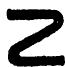
\includegraphics[keepaspectratio]{images/part001_a8399183.jpg}}

Note that for an arbitrary topological space X, property b) does not necessarily imply the existence of a countable base, even if X is compact and every point of X has a countable fundamental system of neighbourhoods (Exercise 13; cf.~Chapter I, § 1, Exercise 7).

PROPOSITION 13. Let X be a topological space which has a countable base \((\mathbf{U}_n)\) ; then for each open covering \((\mathbf{V}_t)_{i \in \mathbf{I}}\) of X there exists a countable subset J of I such that \((\mathbf{V}_t)_{i \in \mathbf{J}}\) is a covering of X.

Let H be the subset of N consisting of indices n such that \(U_{n}\) is contained in at least one of the \(V_{t}\) ; the sequence \((\mathrm{U}_{n})_{n\in\mathbf{H}}\) is a covering of X, because every point \(x\in X\) belongs to some \(V_{t}\) , and since \(V_{t}\) is open, there is an index n such that \(x\in U_{n}\subset V_{t}\) . Hence there is a mapping \(\psi\) of H into I such that \(U_{n}\subset V_{\psi(n)}\) for each \(n\in H\) ; taking \(J=\psi(H)\) , which is countable, the proposition is proved.

\subsection{COMPACT METRIC SPACES; COMPACT METRIZABLE SPACES}

The criterion for precompactness of a uniform space (Chapter II, § 4, no. 2, Theorem 3) gives rise to the following proposition for metric spaces:

PROPOSITION 14. A metric space X is precompact if and only if, for each \(\varepsilon > 0\) , there is a finite covering of X by sets of diameter \(\leqslant \varepsilon\) .

If we adjoin the hypothesis that X is complete we have a criterion for compactness of metric spaces.

From Proposition 14 we get a topological criterion for compactness, applicable to metrizable spaces:

PROPOSITION 15. A metrizable topological space X is compact if and only if every infinite sequence of points of X has a cluster point in X.

Axiom (C) of Chapter I, § 9, no. 1 shows that the condition is necessary. To show sufficiency, let \(d\) be a metric compatible with the topology of \(\mathbf{X}\) . We show first that the metric space \(\mathbf{X}\) so defined is complete: every Cauchy sequence in \(\mathbf{X}\) has a cluster point and is therefore convergent (Chapter II, § 3, no. 2, Proposition 5, Corollary 2); hence \(\mathbf{X}\) is complete, by Proposition 9. Next we shall show that \(\mathbf{X}\) is precompact; if this were not so, then by Proposition 14 there would exist a real number \(\alpha > 0\) such that \(\mathbf{X}\) could not be covered by any finite number of subsets of \(\mathbf{X}\) of diameter \(\leqslant \alpha\) . We could then define by induction on \(n\) an infinite sequence \((x_n)\) of points of \(\mathbf{X}\) by the condition \(d(x_p, x_n) > \frac{1}{2} \alpha\) for all \(p < n\) ; and such a sequence can have no cluster point, since every ball of radius \(< \frac{1}{2} \alpha\) contains at most one point of the sequence.

COROLLARY. A subset A of a metrizable topological space X is relatively compact if and only if every infinite sequence of points of A has a cluster point in X.

Let \(d\) be a metric compatible with the topology of \(\mathbf{X}\) . We shall show that the space \(\overline{\mathbf{A}}\) is compact, by applying the criterion of Proposition 15. Let \((x_{n})\) be a sequence of points of \(\overline{\mathbf{A}}\) ; then for each index \(n\) there exists \(y_{n} \in \mathbf{A}\) such that \(d(x_{n}, y_{n}) < 1/n\) ; the sequence \((y_{n})\) has, by hypothesis, a cluster point \(a \in \mathbf{X}\) , and \(a\) is also a cluster point of the sequence \((x_{n})\) , for if \(y_{m}\) lies in the ball with centre \(a\) and radius \(1/n\) , for some \(m > n\) , then \(x_{m}\) lies in the ball with centre \(a\) and radius \(2/n\) .

It should be remarked that Proposition 15 is not a consequence of the existence of a countable fundamental system of neighbourhoods at each point of X; there are examples of non-metrizable, non-compact spaces in which every point has a countable fundamental system of neighbourhoods and every infinite sequence of points has a cluster point (Exercise 15).

PROPOSITION 16. A compact space X is metrizable if and only if its topology has a countable base.

The condition is necessary. By Proposition 14, for each integer \(n \geqslant 1\) there is a finite subset \(A_n\) of \(X\) such that the distance of \(A_n\) from every point of \(X\) is \(\leqslant 1/n\) ; the countable set \(A = \bigcup_{n} A_n\) is therefore dense in \(X\) , and the result follows from Proposition 12 of no. 8.

The condition is sufficient. Let \((\mathbf{U}_{n})\) be a countable base of the topology of X. Every neighbourhood of a point of the diagonal \(\Delta\) of \(X \times X\) therefore contains a neighbourhood of the form \(U_{n} \times U_{n}\) ; applying the Borel-Lebesgue axiom to the compact subset \(\Delta\) of \(X \times X\) , it follows that every neighbourhood of \(\Delta\) contains a finite union of sets of the form \(U_{n} \times U_{n}\) , which is a neighbourhood of \(\Delta\) . Hence the neighbourhoods of \(\Delta\) which are finite unions of sets of the form \(U_{n} \times U_{n}\) form a fundamental system of entourages of the uniformity of X (Chapter II, § 4, no. 1, Theorem 1), and the result therefore follows from Theorem 1 of no. 4.

COROLLARY. Let X be a locally compact space and let X' be the compact space obtained by adjoining a point at infinity ω to X (Chapter I, § 9, no. 8). Then the following statements are equivalent:

\begin{enumerate}
\def\labelenumi{\alph{enumi})}
\item
  The topology of \(\mathbf{X}\) has a countable base.
\item
  \(\mathbf{X}'\) is metrizable.
\item
  X is metrizable and \(\sigma\) -compact.
\end{enumerate}

a) \(\Longrightarrow\) b): Let \((\mathbf{U}_n)\) be a countable base of the topology of \(\mathbf{X}\) . Each neighbourhood of a point \(x \in \mathbf{X}\) contains a compact neighbourhood of \(x\) , which in turn contains a neighbourhood of \(x\) equal to some \(\mathbf{U}_n\) . Hence the relatively compact \(\mathbf{U}_n\) form a base of the topology of \(\mathbf{X}\) , and we may therefore suppose that all the \(\mathbf{U}_n\) are relatively compact. \(\mathbf{X}\) is therefore a countable union of compact sets \(\overline{\mathbf{U}}_n\) , i.e.~it is \(\sigma\) -compact; this implies that in \(\mathbf{X}'\) the point \(\omega\) has a countable fundamental system \((\mathbf{V}_n)\) of open neighbourhoods (Chapter I, § 9, no. 9, Proposition 15, Corollary 2). Hence each neighbourhood of a point \(y \in \mathbf{X}'\) contains either one of the \(\mathbf{U}_n\) or one of the \(\mathbf{V}_n\) , which is a neighbourhood of \(y\) , and so the \(U_{n}\) and the \(V_{n}\) form a countable base of the topology of \(X'\) . Hence \(X'\) is metrizable, by Proposition 16.

b) \(\Longrightarrow\) c): If \(X'\) is metrizable, then \(\omega\) has a countable fundamental system of neighbourhoods, and therefore \(X\) is \(\sigma\) -compact by Chapter I, § 9, no. 9, Proposition 15, Corollary 2.

c) \(\Longrightarrow a)\) : By hypothesis, there is an increasing sequence \((\mathbf{V}_n)\) of relatively compact open sets which cover \(\mathbf{X}\) and are such that \(\overline{\mathbf{V}}_n \subset \mathbf{V}_{n+1}\) (Chapter I, § 9, no. 9, Proposition 15). The subspace \(\overline{\mathbf{V}}_n\) is compact and metrizable and therefore has a countable base (Proposition 16), and therefore so does \(\mathbf{V}_n\) . Let \((\mathbf{U}_{mn})_{m \geqslant 1}\) be a base of the topology of \(\mathbf{V}_n\) . For each \(x \in \mathbf{X}\) and each neighbourhood \(W\) of \(x\) , there exists \(n\) such that \(x \in \mathbf{V}_n\) , hence there exists \(m\) such that \(x \in \mathbf{U}_{mn} \subset \mathbf{V}_n \cap W\) . Hence the sets \(\mathbf{U}_{mn}\) ( \(m \geqslant 1\) , \(n \geqslant 1\) ) form a base of the topology of \(\mathbf{X}\) .
